% Thesis skeleton. Compile from this folder (Overleaf: upload the repo, set main.tex as the main file).
% Figures are read from ../figures/<stage>/<name>.pdf, written by scripts/*.py.
\documentclass[12pt,a4paper,oneside]{report}
\usepackage[utf8]{inputenc}
\usepackage[T1]{fontenc}
\usepackage{lmodern}
\usepackage[margin=2.5cm]{geometry}
\usepackage{amsmath,amssymb}
\usepackage{graphicx}
\usepackage{booktabs}
\usepackage{multirow}
\usepackage{caption}
\usepackage{xcolor}
% IEEE referencing: numbered [1], [2], ... in order of first citation. IEEEtranN is the natbib-compatible
% IEEEtran style, so \citet{x} still gives "Author et al. [n]" in running text.
\usepackage[numbers,square,comma,sort&compress]{natbib}
\usepackage[hidelinks]{hyperref}
\usepackage[capitalise,noabbrev]{cleveref}

\graphicspath{{../figures/}}
\captionsetup{font=small,labelfont=bf}
\captionsetup[figure]{name=Fig.}                 % IEEE: "Fig. 3"
\crefname{figure}{Fig.}{Figs.}
\Crefname{figure}{Fig.}{Figs.}

\newcommand{\ES}{\mathrm{ES}}
\newcommand{\VaR}{\mathrm{VaR}}
\newcommand{\pct}[1]{#1\%}
% A reference still to be added: renders in red so it cannot slip into the submitted version.
\newcommand{\citeneeded}[1]{\textcolor{red}{[cite: #1]}}

\title{Physics-Informed Neural Networks for Financial Tail-Risk Estimation}
\author{Aditya Siraskar \and Utkarsh Sinha \and Aditya Sharma\\[1ex] Mentor: Dr.\ Jaykrishna Joshi}
\date{}

\begin{document}
\maketitle
\tableofcontents

\chapter{Introduction}
\label{ch:introduction}

\section{Motivation}
Financial institutions are threatened less by ordinary daily fluctuations than by rare, large losses. Their
risk measures therefore concentrate on the tail of the loss distribution: Value at Risk (VaR), the loss level
exceeded with a given small probability, and Expected Shortfall (ES), the average loss beyond that level. Since
the Fundamental Review of the Trading Book, banks compute market-risk capital from the 97.5\% ES
\citep{bcbs2019}, and ES has the theoretical advantage of being a coherent risk measure
\citep{artzner1999,acerbi2002}.

Estimating these quantities is difficult because returns are not Gaussian \citep{mandelbrot1963,cont2001}.
Extreme moves occur far more often than a normal distribution predicts, volatility clusters in time, and
crashes such as March 2020 arrive as sudden jumps rather than as a sequence of ordinary moves. A model can fit
the centre of the return distribution well and still misjudge the worst one percent of outcomes, which is
exactly the part that VaR and ES measure.

Jump-diffusion models \citep{merton1976,kou2002} capture fat tails and crashes by adding a compound Poisson
jump to the diffusion. The density of returns under such a model solves a forward partial
integro-differential equation (PIDE), and both risk measures follow from that density: VaR is one of its
quantiles and ES an integral over its tail. The practical question is how to obtain the density accurately in
the tail, for a portfolio of several assets, and quickly enough to be used when market conditions change.

Classical methods each fail one of these requirements. Finite-difference solvers are accurate in one or two
dimensions but their cost grows exponentially with the number of assets. Monte Carlo scales to any dimension but
its tail estimates converge slowly, as $N^{-1/2}$ in the number of simulated paths, and must be repeated for every
new parameter set. Physics-informed neural networks (PINNs) \citep{raissi2019} offer a third route: a neural
network trained to satisfy the equation itself, which is mesh-free, can take model parameters as inputs, and,
once trained, is evaluated by a forward pass.

\section{Problem statement}
This thesis asks \emph{when a physics-informed neural network gives better tail-risk estimates than
conventional methods, and when its overhead outweighs the gain}. The aim is not to show that PINNs are better,
but to establish whether, when and why they are, with a design in which a negative answer is as informative as a
positive one. That requires an exact ground truth, so that every error is measured rather than estimated; strong
baselines, both numerical (finite differences, Monte Carlo) and statistical (GARCH, filtered historical
simulation, extreme value theory); and an honest accounting of cost.

\section{Research questions}
\begin{description}
  \item[RQ1 (density versus tail).] How accurately does the PINN recover the density in the bulk, and separately
    in the tail? A small average error can hide a large tail error.
  \item[RQ2 (risk accuracy and calibration).] How accurate are the resulting VaR and ES against exact values,
    and how well calibrated are they on real multi-asset data?
  \item[RQ3 (does the physics help?).] How does the PINN compare with the same network trained on data alone,
    and how many samples does the data-only network need to match it?
  \item[RQ4 (scaling with dimension).] How does accuracy and cost change with the number of assets, compared with
    finite differences (usable up to about three dimensions) and Monte Carlo?
  \item[RQ5 (latency).] Can one network, trained across a range of market parameters, answer risk queries faster
    than Monte Carlo at equal tail error, and after how many queries does its training cost pay back?
\end{description}

\section{Approach}
The study proceeds in stages of increasing difficulty, each validated before the next.
\begin{enumerate}
  \item A one-dimensional Merton model, where the exact density, a finite-difference solver and Monte Carlo
    agree to high precision. Here the PINN design is fixed and each of its components is tested by ablation.
  \item A $d$-asset model with one common market-jump factor, which keeps the jump integral one-dimensional and
    the exact density available in every dimension. The PINN is scaled from one to ten assets.
  \item An amortised PINN that takes the market parameters as inputs, so one trained network covers a whole
    range of market states, with a latency comparison against Monte Carlo.
  \item Daily one-day-ahead backtests on two five-asset baskets (NIFTY and S\&P sector ETFs, 2018--2026) against
    seven standard risk models, for a linear and an option portfolio.
  \item An ablation of the physics against a data-only network, and a set of controlled failure cases.
\end{enumerate}

\section{Contributions}
\begin{itemize}
  \item A PINN design for the forward jump-diffusion PIDE that learns the tail as accurately as the bulk: a
    log-density output, a log-form residual that measures relative error, Gauss--Hermite quadrature of the jump
    integral, and a normalisation penalty. Ablations quantify the contribution of each.
  \item A mesh-free extension to $d$ assets in which collocation, normalisation and risk all use one importance
    proposal built from the equation's coefficients, with an exact or stochastic (Hutchinson) trace. It reaches
    about 1\% ES error up to five assets and identifies ten assets as the breakdown point.
  \item An amortised network over volatility level, jump intensity and jump mean, with risk contributions and
    scenario analysis by differentiation, and a latency comparison that reports where Monte Carlo is faster.
  \item A real-data evaluation with Kupiec, Christoffersen, FZ0 and Diebold--Mariano tests in which the PINN's
    error is separated from the model's error by evaluating the same model with its exact density.
  \item A physics-versus-data ablation that measures the value of the equation in exact samples, a set of failure
    cases including a far-tail extrapolation failure and its remedy, and an open, tested and reproducible code
    base in which every figure and number is produced by a configuration-driven script.
\end{itemize}

\section{Scope}
The model is a jump-diffusion with constant coefficients, Gaussian jump sizes and one common jump factor;
time-varying volatility enters through a daily volatility scale. Results are reported for up to five assets,
with ten assets as the documented breakdown point. Stochastic volatility, idiosyncratic jumps and self-exciting
jump arrivals are left to future work.

\section{Outline}
\Cref{ch:literature} reviews tail-risk estimation, jump-diffusion models, physics-informed and other neural PDE
solvers, and identifies the gap. \Cref{ch:methodology} describes the model, the reference methods, the PINN
design and the evaluation protocol. \Cref{ch:results} reports the results stage by stage and answers the research
questions. \Cref{ch:conclusion} summarises the findings, their limitations and directions for further work.

% Literature review. \citeneeded{...} marks claims whose reference the team still has to add
% (they render in red, so none can slip into the submitted version).
\chapter{Literature review}
\label{ch:literature}

This chapter reviews the four bodies of work the thesis connects: tail-risk measures and their estimation
(\cref{sec:lit-risk}), jump-diffusion models and their numerical solution (\cref{sec:lit-jumps}),
physics-informed and other neural PDE solvers (\cref{sec:lit-pinn}), and their use in finance
(\cref{sec:lit-pinnfin}). \Cref{sec:lit-gap} states the gap.

% ------------------------------------------------------------------------------------------------
\section{Tail-risk measures and their estimation}
\label{sec:lit-risk}

\paragraph{VaR and ES.} Value at Risk became the industry standard in the 1990s \citep{jorion2007}. It is a
quantile, and therefore says nothing about the size of losses beyond it; it is also not subadditive, so the VaR of
a portfolio can exceed the sum of its parts. \Citet{artzner1999} defined the axioms of coherent risk measures, and
\citet{acerbi2002} showed that Expected Shortfall satisfies them. The Basel Committee's Fundamental Review of the
Trading Book replaced 99\% VaR with 97.5\% ES for market-risk capital \citep{bcbs2019}.

\paragraph{Estimation methods.} Four families dominate practice.
\begin{itemize}
  \item \textbf{Parametric} models assume a distribution, usually Gaussian or Student-$t$, with volatility from an
    EWMA filter \citep{riskmetrics1996} or a GARCH model \citep{bollerslev1986}. Multivariate versions model
    correlations, for example with dynamic conditional correlation \citep{engle2002}.
  \item \textbf{Historical simulation} uses the empirical distribution of past returns. It makes no distributional
    assumption but reacts slowly to changes in volatility. Filtered historical simulation rescales past returns by
    the ratio of current to past volatility \citep{barone1999}, and is a strong benchmark in comparative studies
    \citeneeded{Bank of England study of filtered-HS VaR, cited in Review 2}.
  \item \textbf{Extreme value theory} fits a generalised Pareto distribution to the tail. \Citet{mcneil2000}
    combine it with GARCH filtering, applying EVT to the standardised residuals.
  \item \textbf{Monte Carlo} simulation from a fitted model handles any model and any portfolio, including
    options, at a cost that grows with the precision required in the tail \citep{glasserman2003}.
\end{itemize}

\paragraph{Backtesting.} \Citet{kupiec1995} tests whether the frequency of VaR breaches matches the nominal
level, and \citet{christoffersen1998} adds a test that breaches are independent over time. Neither evaluates ES.
ES is not elicitable on its own \citep{gneiting2011}, which long made it hard to backtest, but the pair (VaR, ES)
is jointly elicitable \citep{fissler2016}. This gives strictly consistent scoring functions such as the FZ0 loss
of \citet{patton2019}, with which competing forecasts can be ranked, and their differences tested with the
Diebold--Mariano test \citep{diebold1995} using a Newey--West variance \citep{newey1987}.

% ------------------------------------------------------------------------------------------------
\section{Jump-diffusion models}
\label{sec:lit-jumps}

Returns exhibit fat tails, volatility clustering and occasional discontinuities \citep{mandelbrot1963,cont2001}.
\Citet{merton1976} added a compound Poisson process with Gaussian jump sizes to the Black--Scholes diffusion; the
density is then a Poisson mixture of Gaussians, available in closed form. \Citet{kou2002} uses double-exponential
jumps, which give a heavier tail and analytical tractability for path-dependent options. \Citet{cont2004} give a
comprehensive treatment of jump processes in finance, including their generators and the integro-differential
equations they lead to.

The density of a jump-diffusion solves a forward PIDE, the Fokker--Planck equation with an added nonlocal jump
term. It is usually solved by finite differences, treating the local terms implicitly and the jump integral
explicitly, with the convolution computed by FFT \citep{andersen2000,cont2004}. These schemes are accurate and fast
in one dimension, but as with every grid method their cost grows as $n^d$ in $d$ dimensions, which limits them to
two or three assets.

% ------------------------------------------------------------------------------------------------
\section{Neural solvers for PDEs}
\label{sec:lit-pinn}

\paragraph{Physics-informed neural networks.} The idea of training a network to satisfy a differential equation
goes back to \citet{lagaris1998}. \Citet{raissi2019} gave it its current form: a network approximates the solution,
automatic differentiation evaluates the PDE residual at sampled collocation points, and the loss combines the
residual with initial and boundary conditions. PINNs are mesh-free, handle forward and inverse problems in the
same framework and can take parameters as inputs \citep{karniadakis2021}.

\paragraph{Known difficulties.} PINN training is fragile. Loss terms can have very different gradient magnitudes,
which unbalances training \citep{wang2021}, and some problems are not learned at all because of the optimisation
landscape rather than the network's capacity \citep{krishnapriyan2021}. Two difficulties are specific to densities:
a density spans many orders of magnitude, so a residual on $p$ ignores the tail, and the PDE is unchanged by
scaling $p$, so normalisation must be imposed separately.

\paragraph{Fokker--Planck equations.} PINNs have been applied to forward and inverse Fokker--Planck problems
\citep{chen2021fp}, mostly with continuous (diffusive) dynamics. Nonlocal jump terms, which make the equation a
PIDE, are less studied.

\paragraph{High dimensions.} Deep BSDE methods \citep{han2018} and the deep Galerkin method
\citep{sirignano2018} solve PDEs in hundreds of dimensions, typically for a value at one point or for a smooth
solution, not for a density across its tail. In PINNs the cost of second derivatives grows with $d$; Hutchinson's
stochastic trace estimator \citep{hutchinson1989} replaces the full Laplacian by random projections, and has been
used to scale PINNs to high dimensions \citep{hu2024}.

\paragraph{Neural operators and density models.} Neural operators such as DeepONet \citep{lu2021} and the Fourier
neural operator \citep{li2021} learn a map from parameters or initial conditions to solutions, from many solved
examples. The amortised PINN of this thesis targets the same goal, one network for a family of problems, but is
trained from the equation alone, without solved examples. Data-driven density estimators such as normalising
flows \citep{papamakarios2021} learn densities from samples alone; the data-only baseline of this thesis is the
simplest such model, built from the same network as the PINN so that the comparison isolates the physics.

% ------------------------------------------------------------------------------------------------
\section{Neural networks for finance}
\label{sec:lit-pinnfin}

Option pricing has been the main financial application of neural PDE solvers: the deep Galerkin method was
demonstrated on American options \citep{sirignano2018}, deep BSDE methods on high-dimensional pricing
\citep{han2018}, and PINNs on the Black--Scholes equation and on jump-diffusion pricing PIDEs
\citeneeded{PINN option pricing, incl.\ jump-diffusion, cited in Review 2}. These works solve the backward
pricing equation for a price, a smooth function whose accuracy is judged in the bulk. Tail-risk work with neural
networks has mostly been data-driven, using networks to forecast VaR or ES directly from past returns
\citeneeded{neural VaR/ES forecasting, e.g.\ quantile-regression networks}.

% ------------------------------------------------------------------------------------------------
\section{Research gap}
\label{sec:lit-gap}

Applying a PINN to a financial equation is no longer new. What the literature does not provide is a systematic
test of whether PINN-solved \emph{densities} give accurate and useful \emph{tail risk}. Such a test requires:
\begin{itemize}
  \item tail accuracy measured separately from bulk accuracy, against an exact reference;
  \item VaR and ES compared with both numerical solvers (finite differences, Monte Carlo) and the statistical risk
    models used in practice (historical simulation, GARCH, EVT), including joint VaR--ES scoring;
  \item the multi-asset case, where grid solvers cannot be used and a neural solver could add value;
  \item an honest accounting of training cost and query latency against Monte Carlo;
  \item a direct measurement of what the physics contributes over the same network trained on data, and an
    account of where the method fails.
\end{itemize}
This thesis provides that test, for jump-diffusion models with up to five assets and on two real equity baskets.

% Methodology chapter. Settings are those in configs/*.yaml; the implementation is pinn_tailrisk/.
\chapter{Methodology}
\label{ch:methodology}

This chapter describes the model (\cref{sec:met-model}), the reference methods that provide ground truth
(\cref{sec:met-reference}), the physics-informed network in one and in $d$ dimensions
(\cref{sec:met-pinn1d,sec:met-pinnnd}), how risk is read from it (\cref{sec:met-risk}), the amortised
model (\cref{sec:met-amortised}), the real-data study (\cref{sec:met-real}), the data-only baseline
(\cref{sec:met-dataonly}) and the evaluation protocol (\cref{sec:met-eval}). Time is measured in years of
252 trading days and returns are log returns throughout.

% ------------------------------------------------------------------------------------------------
\section{Model}
\label{sec:met-model}

\subsection{One asset}
The log return $X_t$ (with $X_0 = 0$) follows the Merton jump-diffusion
\begin{equation}
  dX_t = a\,dt + \sigma\,dW_t + dJ_t, \qquad J_t = \sum_{i=1}^{N_t} Y_i, \qquad
  N_t \sim \mathrm{Poisson}(\lambda t), \quad Y_i \sim \mathcal{N}(\mu_J, \sigma_J^2).
  \label{eq:merton}
\end{equation}
Its density $p(x,t)$ solves the forward Kolmogorov (Fokker--Planck) partial integro-differential equation
\begin{equation}
  p_t = -a\,p_x + \tfrac12 \sigma^2 p_{xx} + \lambda \int_{\mathbb{R}} p(x - y, t)\, f_Y(y)\,dy - \lambda\, p,
  \label{eq:pide1d}
\end{equation}
with $p(\cdot, 0) = \delta_0$. The exact solution is a Poisson mixture of Gaussians \citep{merton1976},
\begin{equation}
  p(x,t) = \sum_{k \ge 0} \frac{e^{-\lambda t}(\lambda t)^k}{k!}\,
           \mathcal{N}\!\left(x;\; a t + k\mu_J,\; \sigma^2 t + k\sigma_J^2\right),
  \label{eq:exact1d}
\end{equation}
which is what makes the model suitable for a validation study: every PINN output can be compared with an
exact answer. The base parameters, representing an equity index with a crash component, are $a = 0.05$,
$\sigma = 0.20$, $\lambda = 5$/yr, $\mu_J = -0.05$ and $\sigma_J = 0.07$.

\subsection{Several assets with a common jump}
For $d$ assets the diffusion is $\mathcal{N}(a t, \Sigma t)$ and all assets share one market-jump factor:
on a jump every asset moves by $\beta_i Y$ with a scalar $Y \sim \mathcal{N}(\mu_J, \sigma_J^2)$ and fixed
loadings $\beta \in \mathbb{R}^d$. The forward equation becomes
\begin{equation}
  p_t = -a \cdot \nabla p + \tfrac12 \operatorname{tr}\!\big(\Sigma \nabla^2 p\big)
        + \lambda \int_{\mathbb{R}} p(x - \beta y, t)\, f_Y(y)\,dy - \lambda\, p .
  \label{eq:pidend}
\end{equation}
Two properties follow from the common-jump structure. First, the jump integral is one-dimensional in any
dimension, so it can be evaluated by the same quadrature as in 1-D; a full $d$-dimensional jump distribution
would make it a $d$-dimensional integral. Second, the density is again an exact Gaussian mixture, with
component $k$ having mean $a t + k\mu_J\beta$ and covariance $\Sigma t + k\sigma_J^2\beta\beta^\top$.

The family used in the scaling study has volatilities spread linearly over $[0.18, 0.30]$, loadings over
$[0.8, 1.2]$ and equicorrelation $\rho = 0.4$, with the jump parameters of the 1-D model.

\subsection{Why the multi-asset density is needed}
For a linear portfolio with weights $w$, the portfolio log return $w^\top X$ is itself a 1-D Merton process
with drift $w^\top a$, volatility $\sqrt{w^\top \Sigma w}$ and jump $(w^\top \beta)\,Y$. A linear portfolio
alone therefore does not require a $d$-dimensional solver. We use this projection as an exact reference for
linear portfolios, and the joint density for what the projection cannot provide: one density that serves every
portfolio and gives risk contributions by differentiation (\cref{sec:met-amortised}), and non-linear
portfolios that hold options (\cref{sec:met-real}).

% ------------------------------------------------------------------------------------------------
\section{Reference methods}
\label{sec:met-reference}

\paragraph{Closed form.} \Cref{eq:exact1d} and its multivariate version, truncated where the neglected
Poisson mass is negligible, give exact densities. Exact VaR and ES of a linear portfolio come from the 1-D
projection by root finding on the mixture CDF and the closed-form partial expectation of each Gaussian
component.

\paragraph{Finite differences in 1-D.} \Cref{eq:pide1d} is solved by an IMEX scheme: Crank--Nicolson for
drift, diffusion and $-\lambda p$, and second-order Adams--Bashforth for the jump convolution, which is applied
by FFT with a cell-averaged jump kernel so that mass is exact on the grid. The scheme is second order in space
and time. It runs on $[-1.0, 0.5]$ with 4001 points and $p = 0$ at both ends; this domain is wider than the one
the PINN is evaluated on, because on a narrower one the zero boundaries distort the far tail.

\paragraph{Finite differences in 2-D.} For $d = 2$ a Douglas ADI scheme ($\theta = 1/2$) treats the
axis-aligned drift and diffusion implicitly with one tridiagonal sweep per axis, and the mixed derivative and
the jump integral explicitly. The jump kernel lies on the line $\{\beta y\}$; it is sampled finely, spread
bilinearly onto grid offsets (preserving mass) and applied by FFT, so a time step costs $O(n^2 \log n)$. This
solver is a second, independent reference in 2-D and a measurement of how grid cost grows with dimension.

\paragraph{Monte Carlo.} Exact simulation of \cref{eq:merton}: a Poisson number of jumps, then the
Gaussian conditional on it. VaR and ES are the empirical quantile and tail mean.

% ------------------------------------------------------------------------------------------------
\section{The PINN in one dimension}
\label{sec:met-pinn1d}

\paragraph{Output and inputs.} The network $g_\phi$ (four hidden layers of width 64, $\tanh$) returns the
\emph{log} density,
\begin{equation}
  u(x,t) = \log p(x,t) = -\tfrac12 \log(2\pi\sigma^2 t) + c\, g_\phi(z, \tau), \qquad
  z = \frac{x - a t}{\sigma\sqrt{t}}, \qquad
  \tau = 2\,\frac{\log t - \log t_0}{\log T - \log t_0} - 1,
  \label{eq:u1d}
\end{equation}
with output scale $c = 10$. Three reasons motivate this form. The density is positive by construction.
Tail densities of order $10^{-4}$ become numbers of order one, which a network can fit. And in the similarity
variable $z$ the diffusive bulk has unit width at every time, instead of collapsing as $t \to t_0$; the known
Gaussian normaliser is added outside the network.

\paragraph{Log-form residual.} Dividing \cref{eq:pide1d} by $p$ gives an equation for $u$,
\begin{equation}
  r(x,t) = u_t + a\,u_x - \tfrac12\sigma^2\big(u_{xx} + u_x^2\big) - \lambda\,(S - 1), \qquad
  S(x,t) = \int e^{\,u(x-y,t) - u(x,t)}\, f_Y(y)\,dy .
  \label{eq:logres}
\end{equation}
The standard residual (on $p$) weighs a point by the size of the density there, so the tail, where risk is
determined, contributes almost nothing to the loss. The log-form residual measures relative error and weighs a
tail point as much as a bulk point. The residual is multiplied by $t$ to make it dimensionless across the time
range.

\paragraph{Jump integral.} Since $Y$ is Gaussian, $S$ is computed by Gauss--Hermite quadrature with nodes
$y_j = \mu_J + \sqrt{2}\,\sigma_J \xi_j$ and weights $w_j/\sqrt{\pi}$; 48 nodes are used (chosen by the ablation
in the results chapter).

\paragraph{Initial condition.} Training starts at $t_0 = 0.5$ day from the exact density
\cref{eq:exact1d}, which avoids the Dirac delta at $t = 0$. In practice this short-time density would come from
the diffusion approximation plus at most one jump; here it is exact so that the study measures the PDE solve
alone.

\paragraph{Loss.} The loss is
\begin{equation}
  \mathcal{L} = w_{\mathrm{pde}}\,\overline{r^2}
              + w_{\mathrm{ic}}\,\overline{\big(u(x, t_0) - \log p(x, t_0)\big)^2}
              + w_{\mathrm{norm}}\,\overline{\Big(\log \textstyle\int e^{u(x,t)}\,dx\Big)^2}
              + w_{\mathrm{bc}}\,\mathcal{L}_{\mathrm{decay}},
  \label{eq:loss1d}
\end{equation}
with weights 1, 10, 10 and 1. The normalisation term keeps $\int p = 1$, which the residual of
\cref{eq:logres} does not enforce on its own (it is unchanged by adding a constant to $u$). The decay term
asks the density to fall at the ends of the domain $[-0.6, 0.3]$. In 1-D, 4096 collocation points are drawn
per step, 40\% of them around the model's current 1\% quantile (tail-adaptive sampling, refreshed every 250
steps).

\paragraph{Optimisation.} Adam with learning rate $2\times10^{-3}$, cosine-annealed to $2\times10^{-5}$ over
20{,}000 steps, with gradient clipping at norm 1.

% ------------------------------------------------------------------------------------------------
\section{The PINN in $d$ dimensions}
\label{sec:met-pinnnd}

The 1-D design carries over with four changes.

\paragraph{Whitened input.} With $L$ the Cholesky factor of $\Sigma$, the network sees
$z = L^{-1}(x - a t)/\sqrt{t}$ and $\tau$, and the Gaussian normaliser
$-\tfrac12\log\det(2\pi\Sigma t)$ is added to its output. The network has width 128 and depth 4.

\paragraph{Residual.} The log-form residual of \cref{eq:pidend} is
\begin{equation}
  r = u_t + a\cdot\nabla u - \tfrac12\Big[\operatorname{tr}\!\big(\Sigma\nabla^2 u\big)
      + \nabla u^\top \Sigma\, \nabla u\Big] - \lambda (S - 1), \qquad
  S = \int e^{\,u(x - \beta y) - u(x)} f_Y(y)\,dy,
\end{equation}
and $S$ uses the same 48-node quadrature along $\beta$.

\paragraph{Trace term.} $\operatorname{tr}(\Sigma\nabla^2 u) = \sum_i \ell_i^\top \nabla^2 u\, \ell_i$, with
$\ell_i$ the columns of $L$, is computed exactly by $d$ Hessian-vector products for $d \le 4$. For larger $d$ it
is replaced by Hutchinson's estimator $\mathbb{E}_v\big[(Lv)^\top \nabla^2 u\,(Lv)\big]$ with four Rademacher
probes $v$, whose cost does not grow with $d$.

\paragraph{No grid: a proposal built from the coefficients.} A box domain cannot be used in $d$ dimensions,
so collocation, the normalisation integral and the risk computation all draw from a proposal
\begin{equation}
  q(x \mid t) = \sum_{k=0}^{K} \pi_k(t)\; t_\nu\!\Big(x;\; a t + k\mu_J\beta,\;
                c^2\big(\Sigma t + k\sigma_J^2 \beta\beta^\top\big)\Big),
  \label{eq:proposal}
\end{equation}
a mixture over $k = 0,\dots,K$ jumps of multivariate Student-$t$ components. The weights $\pi_k$ are the Poisson
probabilities, floored at 0.05 and renormalised so that every jump count is sampled. The proposal uses only the
coefficients of the PIDE, not its solution. Two versions are used: for collocation and the initial condition,
$\nu = 30$ and $c = 1.5$ (heavier tails put training targets at $\log p \approx -7000$ in high dimension); for
the normalisation integral and for risk, $\nu = 5$ and $c = 1.2$, so that importance weights stay bounded where
the density is non-negligible. The default is $K = 3$ jumps. Tail-adaptive sampling is not used in $d$
dimensions, since it gave no gain in 1-D.

\paragraph{Normalisation loss.} With $M$ proposal draws at each of several times,
\begin{equation}
  \mathcal{L}_{\mathrm{norm}} = \overline{\Big(\log \tfrac1M \textstyle\sum_m e^{\,u(x_m,t) - \log q(x_m \mid t)}\Big)^2},
\end{equation}
computed with a log-sum-exp. Penalising $(\text{mass} - 1)^2$ directly overflows for an untrained network.
The loss weights, optimiser and schedule are those of the 1-D model, with 2048 collocation points, 4096
initial-condition points and 4096 normalisation draws per step.

% ------------------------------------------------------------------------------------------------
\section{Risk from the network}
\label{sec:met-risk}

The loss is $L = -X$ and, at confidence level $\alpha$,
$\VaR_\alpha = \inf\{\ell : P(L \le \ell) \ge \alpha\}$ and $\ES_\alpha = \mathbb{E}[L \mid L \ge \VaR_\alpha]$,
both reported as positive numbers. In 1-D they are read from the density on a grid. In $d$ dimensions they are
computed by self-normalised importance sampling: draws $x_m \sim q(\cdot \mid t)$ from \cref{eq:proposal} get
weights $\tilde w_m \propto \exp\big(u(x_m,t) - \log q(x_m \mid t)\big)$, and VaR and ES of any portfolio
$P\&L(x)$ are the weighted quantile and the weighted tail mean of $P\&L(x_m)$, with the atom at the quantile
split exactly. The same draws serve every portfolio. Because the density is an explicit function of $x$, $w$
and (in the amortised model) the market parameters, risk contributions $\partial\ES/\partial w_i$ follow from
the weighted tail average of each asset's return.

\paragraph{Trust region.} The network is constrained only where collocation points are drawn. Far outside that
region it can decay more slowly than the proposal, and a single draw then dominates the weights. For the
real-data study, draws whose Mahalanobis radius to the nearest collocation component exceeds $r_{\max} = 6$ are
given zero weight; the exact mass removed in this way is below $10^{-15}$.

% ------------------------------------------------------------------------------------------------
\section{Amortised model}
\label{sec:met-amortised}

To answer queries for a changing market without retraining, the network takes the parameters
$\theta = (s, \lambda, \mu_J)$ as additional inputs. Here $s$ multiplies every diffusion volatility
(covariance $s^2\Sigma$, with correlations and loadings fixed), $\lambda$ is the jump intensity and $\mu_J$
the mean jump; $\sigma_J$ is fixed. The whitened input is also divided by $s$. Training draws a fresh $\theta$
for every collocation, initial-condition and normalisation point, from the box $s \in [0.6, 1.6]$,
$\lambda \in [1, 15]$/yr (log-uniform) and $\mu_J \in [-0.10, -0.02]$. The initial condition is the exact mixture
at $t_0$ evaluated at each point's $\theta$, and the proposal of \cref{eq:proposal} is evaluated at each row's
$\theta$. The exact trace is used, and training runs for 30{,}000 steps.

Latency is measured on the same device for PINN importance sampling with $N_{\mathrm{IS}}$ draws and Monte
Carlo with $N_{\mathrm{MC}}$ paths. Fitting error $\propto N^{\text{slope}}$ and latency $\approx l_0 + l_1 N$
for each method gives the cost of each at the PINN's error level, and from that the number of queries at which
the training cost is paid back (the break-even).

% ------------------------------------------------------------------------------------------------
\section{Real-data study}
\label{sec:met-real}

\paragraph{Data.} Two five-asset baskets: the five largest NIFTY 50 constituents (Reliance, HDFC Bank, Infosys,
ICICI Bank, TCS) and five S\&P 500 sector ETFs (XLK, XLF, XLE, XLV, XLI). Daily adjusted prices from Yahoo
Finance from January 2006 (earlier NIFTY prices contain bad prints) to October 2026. The log returns are
committed with the code, since the provider revises adjusted prices. Models are developed on 2006--2017 and
tested from January 2018, which includes the COVID crash.

\paragraph{Calibration.} The common-jump model is fitted by maximum likelihood to daily returns, each day being
one draw of $X$ over one trading day with density the Poisson mixture over $k \le 8$ jumps. In the
\emph{filtered} model a daily volatility scale $s_t$ from an EWMA filter (decay 0.94) multiplies every diffusion
volatility, which is exactly the parameter the amortised PINN takes as input. Jump loadings are fixed equal: with
free loadings the NIFTY jump attaches to a single stock and stops being a market jump. Parameters are optimised
jointly with L-BFGS in double precision, and standard errors come from the inverse Hessian. During the test
period $(\lambda, \mu_J)$ are refitted monthly on a 1000-day window with a Gaussian prior centred on the
development fit (standard deviation 0.5 for $\log\lambda$ and 0.01 for $\mu_J$), because the rolling fit alone is
weakly identified. An \emph{unfiltered} model (no $s_t$, all parameters refitted monthly) is a separate
benchmark.

\paragraph{The PINN.} One amortised network per market is trained on a box set from development data only:
$s$ over the range seen in development (widened by factors 0.75 and 1.35), $\lambda$ within a factor $e^{\pm1.5}$ of
the development fit and $\mu_J$ within $\pm 0.025$. Time runs over $[0.5, 1.5]$ days, since only one-day-ahead
forecasts are needed, and $K = 8$ jumps are allowed because real-data jumps are small and frequent. Each test day
is one forward query at that day's $\theta_t$, using 32{,}768 importance draws. The same model evaluated with its
exact density on the same draws is reported alongside, so the difference between the two is the PINN's error
and not the model's.

\paragraph{Portfolios.} An equal-weight basket (linear) and the basket plus a short one-month put struck 3\%
out of the money, rolled monthly (non-linear). The put is priced by Black--Scholes with zero rate and implied
volatility equal to the EWMA volatility of the basket, and the book is fully revalued on every scenario.

\paragraph{Benchmarks.} All forecast one day ahead without look-ahead: Gaussian (250-day window), historical
simulation (500 days), filtered historical simulation (per-asset EWMA rescaling), GARCH(1,1) with Student-$t$
innovations (1000-day window, refitted monthly), GARCH-EVT \citep{mcneil2000} with a generalised Pareto tail
above the 10\% threshold of the standardised residuals, and DCC-GARCH-$t$ (univariate GARCH refitted monthly,
DCC parameters yearly). Multivariate models produce joint scenarios, so they revalue the non-linear book too.

% ------------------------------------------------------------------------------------------------
\section{Data-only baseline}
\label{sec:met-dataonly}

To measure what the physics contributes (RQ3), the $d$-dimensional network is trained without the PIDE. It is
identical to the PINN in architecture, optimiser, learning-rate schedule, number of steps and normaliser
estimator, and it is trained by maximum likelihood on $N$ exact samples $(x_i, t_i)$:
\begin{equation}
  \mathcal{L}_{\mathrm{NLL}} = -\frac1N \sum_i \Big[u(x_i, t_i) - \log Z(t_i)\Big], \qquad
  \log Z(t) = \log \mathbb{E}_{q}\!\Big[e^{\,u(X,t) - \log q(X \mid t)}\Big],
\end{equation}
where $\log Z$ is estimated on fresh proposal draws at every step, exactly as the PINN's normalisation term.
The samples are spread evenly over 16 times: 13 log-spaced in $[t_0, T]$ plus the three evaluation horizons.
20\% are held out, and the state with the best validation likelihood (on fixed proposal draws) is kept. $N$
ranges over $10^3$, $10^4$, $10^5$ and $10^6$, with three seeds each. Monte Carlo on the same samples (those at
each horizon) is reported as the purely empirical alternative.

% ------------------------------------------------------------------------------------------------
\section{Evaluation protocol}
\label{sec:met-eval}

\paragraph{Portfolios.} For each dimension: the equal-weight portfolio, 15 long-only portfolios with
Dirichlet(1) weights and 4 long--short portfolios (weights summing to one), with a fixed seed. Errors are
reported as the median over these 20 portfolios.

\paragraph{Accuracy.} The headline metric is the relative error of $\ES_{99}$ at 1, 5 and 10 days against the
exact value; VaR and the 97.5\% level are also reported. Density accuracy is split into bulk and tail, which
answers RQ1 directly. In 1-D the bulk error is the relative $L^1$ error between the 1\% and 99\% quantiles and the
tail error the mean absolute error of $\log p$ beyond them. In $d$ dimensions both are evaluated on exact samples:
the mean absolute error of $\log p$ over all samples, and over the samples in the 1\% loss tail of the equal-weight
portfolio.

\paragraph{Sampling controls.} Importance sampling adds sampling error to the network's error. Two controls are
computed on the same draws: the same estimator with the \emph{exact} density (the IS floor, the best any density
could do with this proposal and budget), and Monte Carlo with the same number of draws. All methods in a
comparison use common random numbers, so differences between them are model differences.

\paragraph{Backtests.} For each forecast series, with a breach on day $t$ when the realised P\&L is below
$-\VaR_t$:
\begin{itemize}
  \item \textbf{Kupiec} unconditional coverage: likelihood-ratio test that the breach rate is $1 - \alpha$.
  \item \textbf{Christoffersen} conditional coverage: Kupiec plus a test that breaches are independent from one
        day to the next (a first-order Markov alternative).
  \item \textbf{FZ0} score of \citet{patton2019}, a strictly consistent scoring function for the pair
        (VaR, ES): with $v_t = -\VaR_t$, $e_t = -\ES_t$ and $p = 1-\alpha$,
        \begin{equation}
          S(y_t; v_t, e_t) = -\frac{\mathbf{1}\{y_t \le v_t\}(v_t - y_t)}{p\, e_t} + \frac{v_t}{e_t} + \log(-e_t) - 1,
        \end{equation}
        averaged over the test period (lower is better). It is the only one of these criteria that evaluates ES.
  \item \textbf{Diebold--Mariano} test of equal mean FZ0 loss between each benchmark and the PINN, with a
        Newey--West variance.
\end{itemize}

\paragraph{Failure cases.} Each failure experiment changes one setting of the $d = 2$ model and keeps all
others: a crisis jump intensity $\lambda = 50$/yr with the default proposal ($K = 3$, which leaves 14\% of the
10-day mass in states with more jumps) and with $K = 10$, and a start time ten times closer to the singular
initial condition ($t_0 = 0.05$ day). A far-tail probe evaluates $\log p - \log q$ for the PINN and the exact
density along 2000 random directions up to 150 whitened units.

\paragraph{Reproducibility.} Every experiment is a script driven by a YAML configuration. Each run writes its
figures, its metrics and the code version, library versions and device that produced them. The notebooks only
call these scripts, and the test suite checks the exact density, the reference solvers, the PINN residual
(which vanishes for the exact density as the quadrature is refined) and the data-only likelihood.

% Results chapter. Every number below is read from results/<stage>/metrics.json (or the CSV named
% in the caption) at commit a72fd40; figures are figures/<stage>/<name>.pdf.
\chapter{Results}
\label{ch:results}

This chapter reports the experiments in the order of the research plan: validation in one dimension
(\cref{sec:res-1d}), the multi-asset ground truth (\cref{sec:res-ref2d}), scaling of the PINN with the
number of assets (\cref{sec:res-scaling}), the amortised real-time model (\cref{sec:res-amortised}),
real-data backtests (\cref{sec:res-real}) and the physics-versus-data ablation with the failure cases
(\cref{sec:res-ablation}). \Cref{sec:res-summary} collects the results into one scorecard and answers the
research questions.

\section{Common protocol}
\label{sec:res-protocol}

\paragraph{Model and horizons.} Log returns follow the Merton jump-diffusion of \cref{ch:methodology}
(base parameters $a = 0.05$, $\sigma = 0.20$, $\lambda = 5$/yr, $\mu_J = -0.05$, $\sigma_J = 0.07$). In $d$
dimensions the assets share one market-jump factor with loadings $\beta$, so the exact density is a
Gaussian mixture over the number of jumps and is available in every dimension. The PINN is trained on
$t \in [t_0, T]$ with $t_0 = 0.5$ day and $T = 10$ days, and risk is reported at 1, 5 and 10 days.

\paragraph{Ground truth.} For a linear portfolio $w$, the portfolio log return $w^\top X$ is itself a
one-dimensional Merton process, so its VaR and ES are computed exactly from the 1-D projection. This gives an
exact reference for every portfolio in every dimension, independent of the methods under test.

\paragraph{Risk from the PINN.} The network outputs an unnormalised log density $u(x,t)$. VaR and ES are
computed by self-normalised importance sampling: $N_{\mathrm{IS}} = 262{,}144$ draws from a Student-$t$
mixture proposal $q$ (degrees of freedom 5, one component per jump count $k \le 3$), weighted by
$\exp(u - \log q)$. Two controls separate model error from sampling error:
\begin{itemize}
  \item \textbf{IS floor}: the same draws weighted by the \emph{exact} density. Its error is the smallest
        error any density can reach with this proposal and budget.
  \item \textbf{Monte Carlo at the same $N$}: plain simulation with the same number of draws.
\end{itemize}

\paragraph{Error metric.} The headline metric is the relative ES error
$|\widehat{\ES}_\alpha / \ES_\alpha - 1|$ at $\alpha = 99\%$ (written ES$_{99}$), reported as the median over
20 portfolios per dimension (equal weight, 15 random long-only, 4 long--short). Density accuracy is reported
separately in the bulk and in the tail (mean absolute error of $\log p$ in the 1\% loss tail), which is the
distinction asked for in RQ1 (\cref{sec:met-eval}).

\paragraph{Hardware.} Training ran on a single NVIDIA T4 (Colab for Stages 2--6, Kaggle for Stage 7), with
peak memory below 0.5\,GB in every run.

% ------------------------------------------------------------------------------------------------
\section{One-dimensional validation}
\label{sec:res-1d}

\subsection{Reference solvers}
The finite-difference (FD) solver of the forward PIDE and Monte Carlo were validated against the Merton
closed form before being used as baselines (\cref{fig:ref1d}). On a 4001-point grid the FD solver
reproduces every VaR and ES between 95\% and 99.9\% with relative error below $2\times10^{-4}$ in 0.4\,s,
and its $L^1$ error falls at second order in the grid spacing. Monte Carlo reaches a median ES$_{99}$ error
of 0.6\% with $10^5$ draws and converges at the expected rate $N^{-1/2}$. One correction was needed: the FD
reference must use a wider domain ($[-1.0, 0.5]$ in log return) than the PINN, because its $p = 0$
boundaries otherwise distort the far tail.

\begin{figure}[t]
  \centering
  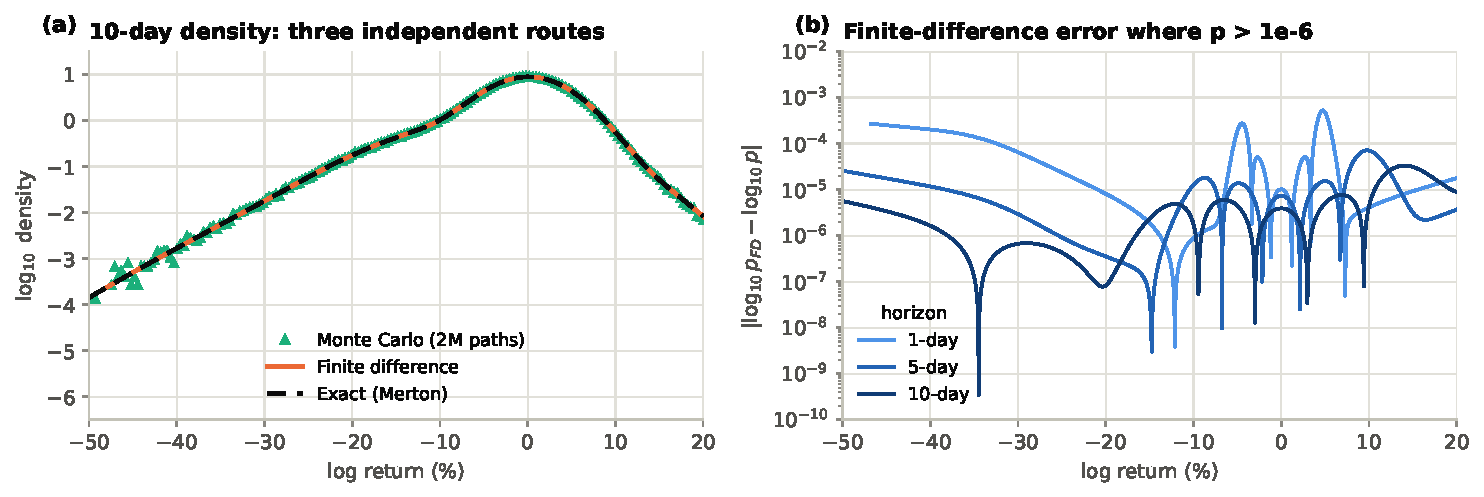
\includegraphics[width=\linewidth]{stage2_reference/fig02_fd_mc_validation.pdf}
  \caption{Stage 2 reference solvers against the Merton closed form: FD and Monte Carlo densities and their
    errors. FD is used as the 1-D baseline from here on.}
  \label{fig:ref1d}
\end{figure}

\subsection{The 1-D PINN}
With 48 Gauss--Hermite nodes for the jump integral the 1-D PINN reaches relative errors below 1\% for every
VaR and ES at 95--99.9\% and all three horizons (maximum 0.61\%). ES$_{99}$ errors are 0.30\%, 0.42\% and
0.16\% at 1, 5 and 10 days (\cref{fig:pinn1d}). The tail is learned as well as the bulk: the left-tail
mean absolute error in $\log p$ is 0.015 at 1 day. Training takes 8.6 minutes and a full density query
1.4\,ms. In one dimension the FD solver is both more accurate (errors of order $10^{-6}$) and faster
(0.34\,s), so the 1-D study validates the method rather than motivating it.

\begin{figure}[t]
  \centering
  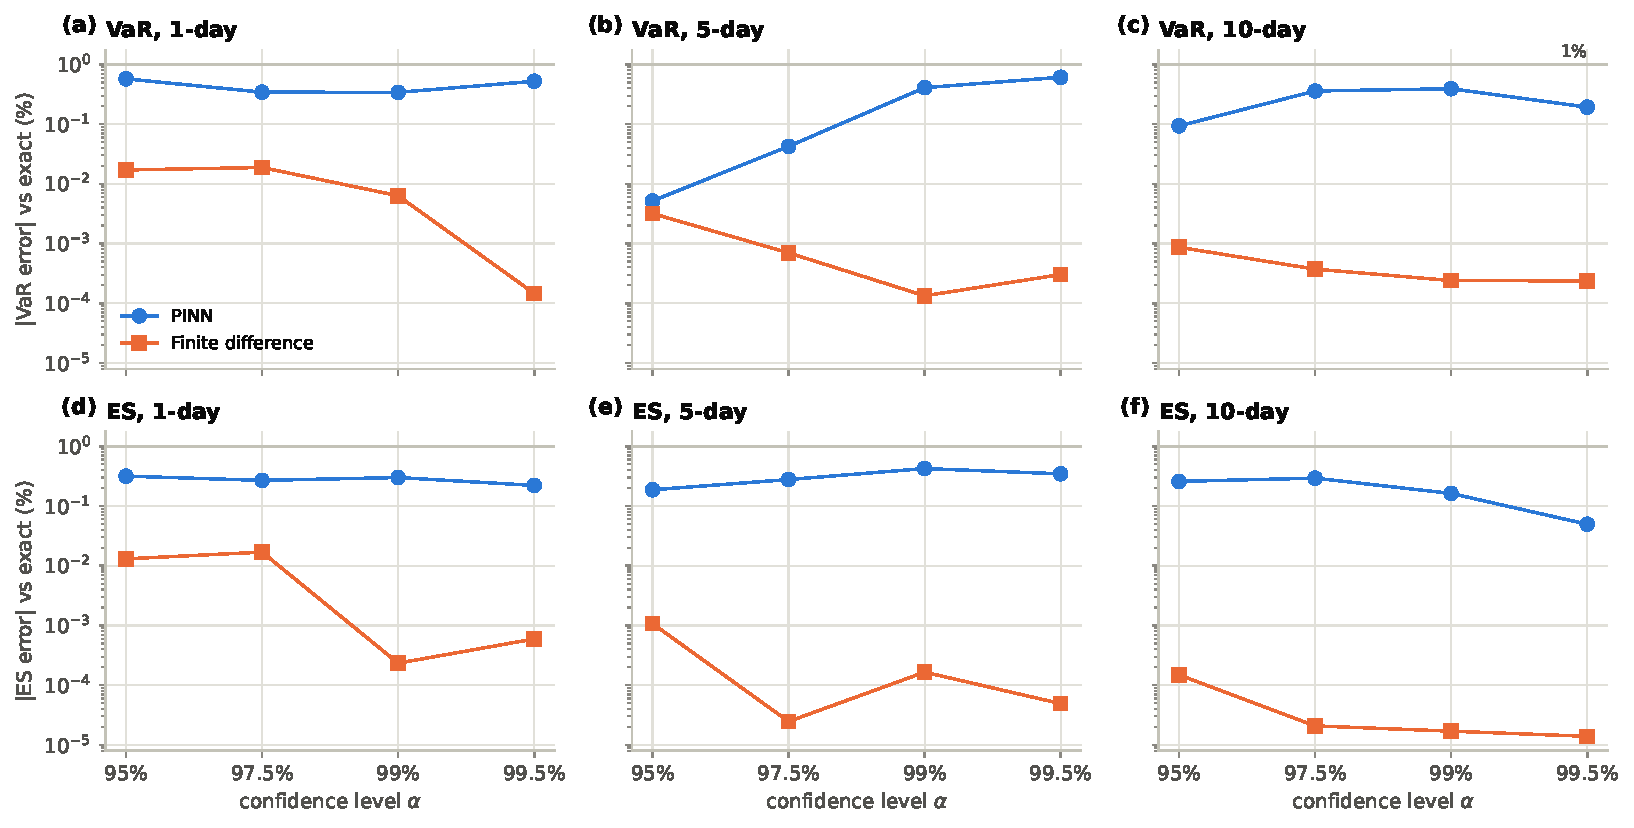
\includegraphics[width=\linewidth]{stage2_pinn1d/fig05_var_es_error.pdf}
  \caption{1-D PINN: relative VaR and ES error against the closed form, by confidence level and horizon.}
  \label{fig:pinn1d}
\end{figure}

\subsection{Ablations}
\Cref{tab:ablation} removes one design choice at a time, with three seeds each. Three components are
essential. The \emph{log-form residual} (writing the PIDE for $\log p$ rather than $p$) is the largest
single factor: without it, 10-day ES errors exceed 50\%. The \emph{resolution of the jump quadrature} sets
the short-horizon accuracy: at 1 day the error falls from 12--15\% with 8 nodes to about 2\% with 24 and
0.2--0.3\% with 48. The \emph{normalisation penalty} is needed at short horizons (2.2\% without it). Tail-adaptive
collocation, by contrast, gave no measurable gain and was dropped from Stage 4 onwards.

\begin{table}[t]
  \centering
  \caption{1-D ablations: ES$_{99}$ relative error, range over three seeds
    (\texttt{results/stage2\_ablation\_seeds.csv}).}
  \label{tab:ablation}
  \begin{tabular}{lcc}
    \toprule
    Variant & 1 day & 10 days \\
    \midrule
    Baseline (log residual, 48 nodes, normalisation) & 0.18--0.30\% & 0.06--0.16\% \\
    Linear residual (on $p$)                         & 0.9--22\%    & 57--152\% \\
    8 quadrature nodes                               & 12--15\%     & 0.2--0.8\% \\
    24 quadrature nodes                              & 1.7--2.1\%   & 0.01--0.18\% \\
    No normalisation penalty                         & 2.1--2.2\%   & 0.07--0.14\% \\
    No tail-adaptive collocation                     & 0.06--0.36\% & 0.04--0.05\% \\
    \bottomrule
  \end{tabular}
\end{table}

% ------------------------------------------------------------------------------------------------
\section{Multi-asset ground truth}
\label{sec:res-ref2d}

For $d = 2$ a Douglas ADI finite-difference scheme with an FFT line kernel for the common jump was built as
an independent check of the closed form. It converges at second order ($L^1$ error 0.027 on a $101^2$ grid,
0.0068 on $201^2$) and reproduces portfolio ES within 0.012\% (Monte Carlo: 0.3\%). Its cost, however, grows
from 0.3\,s for the 1-D grid to 55\,s for a $401^2$ grid, and a $d$-dimensional grid grows as $n^d$
(\cref{fig:fdcost}). Beyond three assets grid methods are not usable, and Monte Carlo and the closed form are
the only references in the scaling study.

\begin{figure}[t]
  \centering
  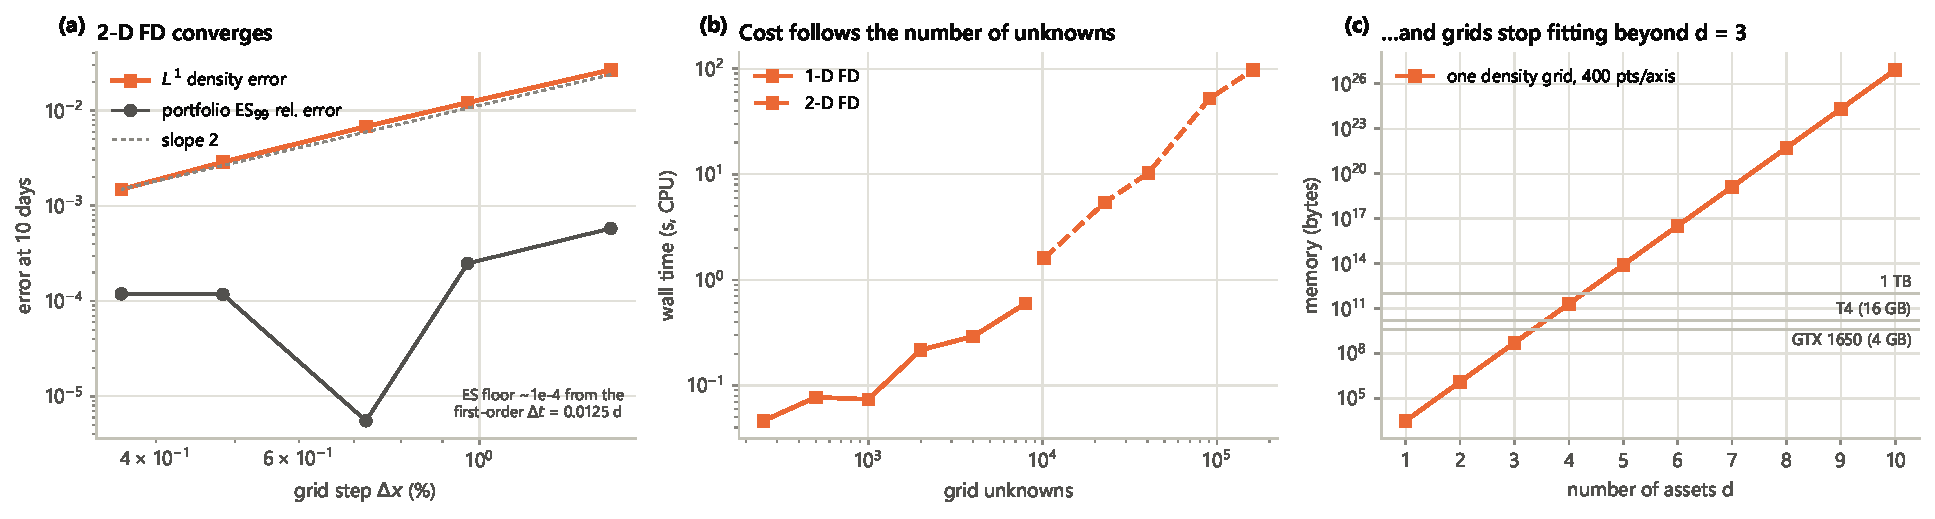
\includegraphics[width=\linewidth]{stage3_multiasset_reference/fig02_fd_cost.pdf}
  \caption{Cost and accuracy of the 2-D FD reference against grid size; the 1-D solver for comparison.}
  \label{fig:fdcost}
\end{figure}

% ------------------------------------------------------------------------------------------------
\section{Scaling with dimension (RQ1, RQ4)}
\label{sec:res-scaling}

The $d$-dimensional PINN uses the same network (width 128, depth 4) and 20{,}000 steps for every $d$. The
Laplacian is computed exactly for $d \le 2$ and with Hutchinson's estimator for $d \ge 5$.
\Cref{tab:scaling} and \cref{fig:scaling} report the result.

\begin{table}[t]
  \centering
  \caption{Scaling with dimension: median ES$_{99}$ error over 20 portfolios, the IS floor and Monte Carlo
    at the same budget, the tail log-density error at 1 day, and training time on a T4
    (\texttt{results/stage4\_summary.csv}).}
  \label{tab:scaling}
  \begin{tabular}{llcccccc}
    \toprule
    $d$ & trace & \multicolumn{2}{c}{PINN} & \multicolumn{2}{c}{MC (same $N$)} & tail MAE & train \\
        &       & 1 day & 10 days & 1 day & 10 days & $\log p$ & (min) \\
    \midrule
    1  & exact      & 1.4\% & 0.05\% & 1.1\% & 0.22\% & 0.03 & 9.4 \\
    2  & exact      & 0.7\% & 1.0\%  & 1.4\% & 1.6\%  & 0.02 & 10.5 \\
    5  & Hutchinson & 1.1\% & 0.6\%  & 0.2\% & 0.4\%  & 0.05 & 12.8 \\
    5  & exact      & 0.09\% & 1.4\% & 0.2\% & 0.4\%  & 0.14 & 13.6 \\
    10 & Hutchinson & 5.2\% & 62\%   & 0.6\% & 0.8\%  & 0.20 & 13.3 \\
    \bottomrule
  \end{tabular}
\end{table}

Up to five assets the PINN stays at or below about 1\% ES$_{99}$ error, within the range of Monte Carlo at
the same budget, with training time almost flat in $d$ (9.4 to 13.6 minutes). Hutchinson's estimator is
as accurate as the exact trace at $d = 5$, so the cost of the Laplacian is not the limit.

At $d = 10$ the method breaks: the PDE loss stalls at 0.76 (0.14 at $d = 5$), and the learned density is
too wide along the jump direction $\beta$ while remaining correct across it. The error grows with horizon,
from 5\% at 1 day to 62\% at 10 days. Following the fallback in the research plan, $d = 10$ is reported as
the breakdown point of this architecture and training budget, and the later stages use $d \le 5$.

\begin{figure}[t]
  \centering
  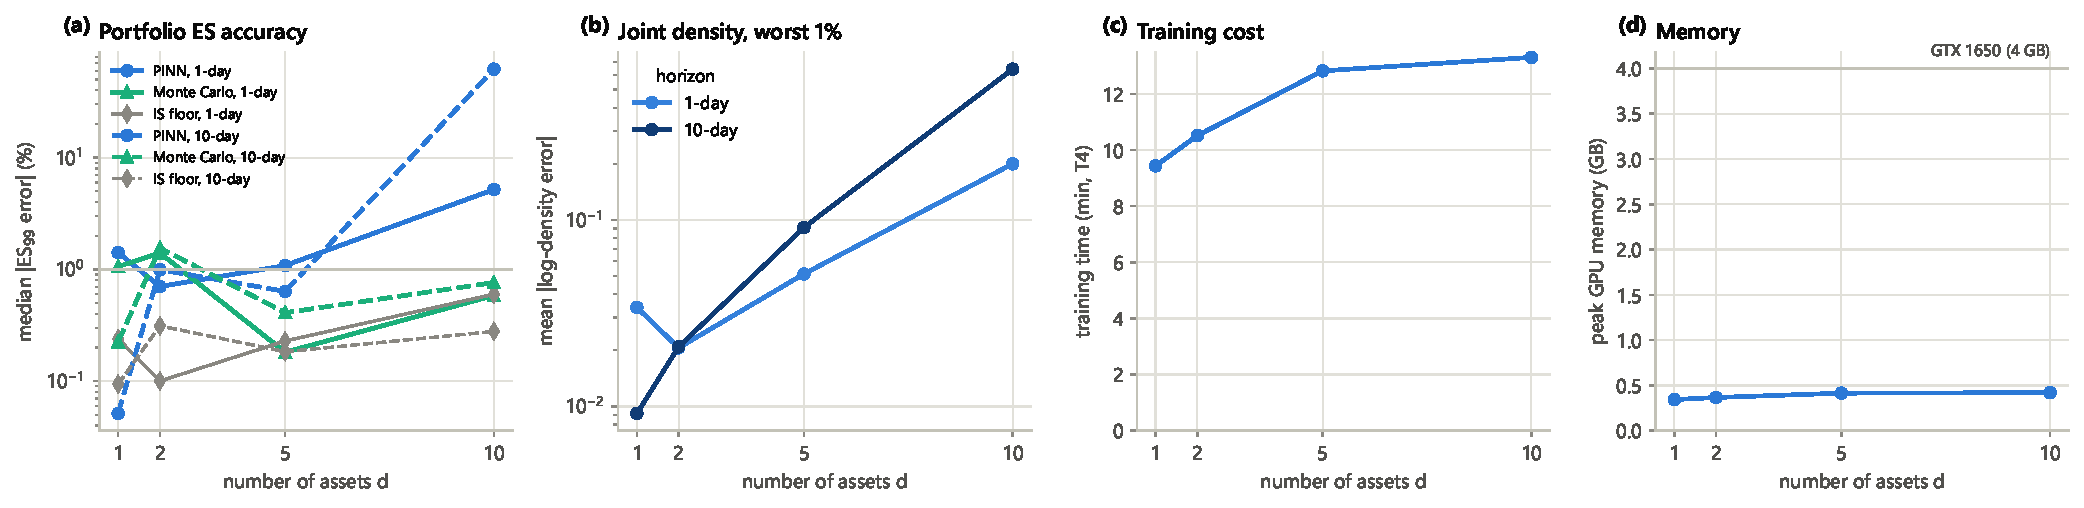
\includegraphics[width=\linewidth]{stage4_summary/fig01_scaling.pdf}
  \caption{ES$_{99}$ error against dimension for the PINN, Monte Carlo at the same budget and the IS floor.}
  \label{fig:scaling}
\end{figure}

% ------------------------------------------------------------------------------------------------
\section{Amortised real-time risk (RQ5)}
\label{sec:res-amortised}

The amortised PINN takes the model parameters $\theta = (s, \lambda, \mu_J)$ as additional inputs: a
volatility multiplier $s \in [0.6, 1.6]$, a jump intensity $\lambda \in [1, 15]$/yr and a mean jump size
$\mu_J \in [-0.10, -0.02]$. One network trained once (18 minutes at $d = 2$, 22 minutes at $d = 5$) then
answers risk queries for any $\theta$ in this box without retraining.

\paragraph{Accuracy over $\theta$.} Over the $(s, \lambda)$ evaluation grid the median ES$_{99}$ error at
1/5/10 days is 1.3/0.8/0.7\% at $d = 2$, against 1.8/0.9/0.8\% for Monte Carlo at the same $N$. At $d = 5$
it is 1.3/1.8/3.4\% against 1.4/0.9/0.7\%: the amortised model matches Monte Carlo at 1 day but degrades with
horizon, and its worst cells reach 10\% (10 days, $s = 0.6$, $\lambda = 15$) and 7\% (high $s$, low
$\lambda$) (\cref{fig:amortised}).

\paragraph{Sensitivities.} Because the density is a differentiable function of $w$ and $\theta$, Euler
risk contributions $\partial \ES / \partial w_i$ and what-if curves come from one model. Euler contributions
agree with finite differences of the exact ES to within about 5\%. ES($\lambda$) follows the exact curve;
ES($s$) has a bias of up to 1.3 percentage points at intermediate $s$.

\paragraph{Latency.} At matched error Monte Carlo is faster: 0.9--1.6\,ms per query against 4--18\,ms
for PINN importance sampling, so the break-even analysis finds no query count at which the PINN pays back
its training cost. This is expected for Merton, where exact simulation costs no more than drawing from the
proposal. The value of the amortised PINN under this model is therefore a smooth, differentiable surrogate in
$\theta$ (for sensitivities and scenario analysis), not raw speed. A speed advantage requires a model whose
simulation is expensive, which is outside the scope of this work.

\begin{figure}[t]
  \centering
  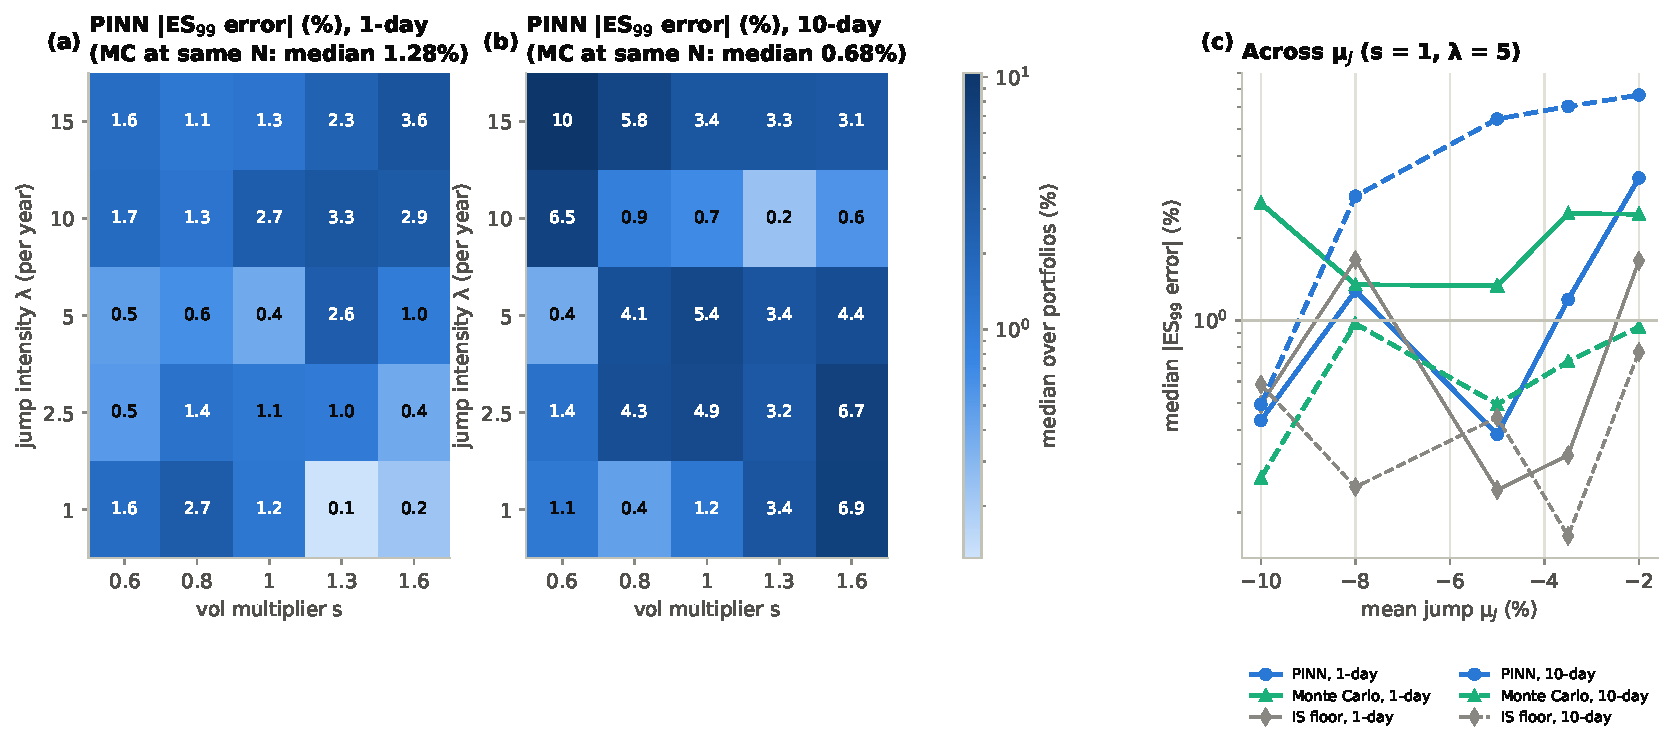
\includegraphics[width=\linewidth]{stage5_amortised_d5/fig02_accuracy_theta.pdf}
  \caption{Amortised PINN at $d = 5$: ES$_{99}$ error over the $(s, \lambda)$ grid at each horizon.}
  \label{fig:amortised}
\end{figure}

% ------------------------------------------------------------------------------------------------
\section{Real-data backtests (RQ2)}
\label{sec:res-real}

\paragraph{Setup.} Two five-asset baskets are used: NIFTY (Reliance, HDFC Bank, Infosys, ICICI Bank, TCS)
and S\&P sector ETFs (XLK, XLF, XLE, XLV, XLI). Daily data run from January 2006 to October 2026; models are
developed on data up to December 2017 and tested from January 2018 (2,176 and 2,217 test days, including the
COVID crash). The filtered Merton model has a daily volatility scale from EWMA filtering and jump parameters
fitted by maximum likelihood, with MAP shrinkage of the rolling $(\lambda, \mu_J)$ towards the development fit.
The PINN is trained once per market over the box of parameters seen in development, then queried every day.
It is compared with Gaussian, historical simulation (HS), filtered HS (FHS), GARCH-$t$, EVT, DCC and an
unfiltered Merton model, on a linear basket and on a non-linear book (basket plus a short 3\%-out-of-the-money
one-month put).

\paragraph{Calibration findings.} Real-data jumps are small and frequent: $\lambda \approx 20$/yr with
$\sigma_J = 2.4\%$ for NIFTY and $\lambda \approx 100$/yr with $\sigma_J = 0.9\%$ for S\&P. They act as a
variance mixture rather than as rare crashes.

\paragraph{The PINN reproduces its model.} Against the exact filtered-Merton density on the same importance
draws, the PINN's daily ES error has median (maximum) 2.8\% (7\%) on NIFTY and 0.2\% (1.7\%) on S\&P at 99\%,
and breach counts are identical (\cref{tab:backtest}). One failure required a fix. On 2022-06-16 a single
proposal draw about 100 standard deviations out received all the importance weight, because the PINN, never
trained there, decays more slowly than the proposal. Draws more than six radii from the nearest collocation
component are now discarded. This removes at most $2\times10^{-16}$ of exact mass and at most 0.9\% of draws,
and keeps the effective sample size above 54\%. The cause is examined in \cref{sec:res-failure}.

\begin{table}[t]
  \centering
  \caption{Linear-basket backtests at 99\%, January 2018 -- October 2026, sorted by the FZ0 joint
    VaR--ES score (lower is better). $p_{\mathrm{uc}}$: Kupiec; $p_{\mathrm{cc}}$: Christoffersen;
    $p_{\mathrm{DM}}$: Diebold--Mariano test of FZ0 against the PINN
    (\texttt{results/stage6\_realdata\_*/backtest.csv}).}
  \label{tab:backtest}
  \small
  \begin{tabular}{llrrrrrr}
    \toprule
    Market & Model & Breaches & Rate & $p_{\mathrm{uc}}$ & $p_{\mathrm{cc}}$ & FZ0 & $p_{\mathrm{DM}}$ \\
    \midrule
    \multirow{9}{*}{NIFTY}
      & DCC             & 28 & 1.29\% & 0.20 & 0.29 & $-3.301$ & 0.004 \\
      & FHS             & 19 & 0.87\% & 0.54 & 0.31 & $-3.278$ & 0.14 \\
      & GARCH-$t$       & 31 & 1.42\% & 0.06 & 0.13 & $-3.205$ & 0.38 \\
      & EVT             & 26 & 1.19\% & 0.38 & 0.41 & $-3.201$ & 0.36 \\
      & \textbf{PINN}   & 15 & 0.69\% & 0.12 & 0.27 & $-3.156$ & -- \\
      & Merton (exact)  & 15 & 0.69\% & 0.12 & 0.27 & $-3.134$ & -- \\
      & HS              & 26 & 1.19\% & 0.38 & 0.008 & $-3.016$ & 0.05 \\
      & Gaussian        & 38 & 1.75\% & 0.002 & $<$0.001 & $-2.881$ & 0.12 \\
      & Merton (unfilt.) & 25 & 1.15\% & 0.50 & $<$0.001 & $-2.672$ & 0.10 \\
    \midrule
    \multirow{9}{*}{S\&P}
      & EVT             & 20 & 0.90\% & 0.64 & 0.04 & $-3.353$ & 0.04 \\
      & GARCH-$t$       & 32 & 1.44\% & 0.05 & 0.03 & $-3.322$ & 0.06 \\
      & DCC             & 33 & 1.49\% & 0.03 & $<$0.001 & $-3.294$ & 0.07 \\
      & FHS             & 20 & 0.90\% & 0.64 & 0.04 & $-3.244$ & 0.14 \\
      & \textbf{PINN}   & 27 & 1.22\% & 0.32 & 0.009 & $-3.046$ & -- \\
      & Merton (exact)  & 27 & 1.22\% & 0.32 & $<$0.001 & $-3.044$ & -- \\
      & HS              & 30 & 1.35\% & 0.11 & $<$0.001 & $-2.731$ & 0.004 \\
      & Merton (unfilt.) & 36 & 1.62\% & 0.007 & $<$0.001 & $-2.533$ & 0.02 \\
      & Gaussian        & 59 & 2.66\% & $<$0.001 & $<$0.001 & $-2.297$ & 0.01 \\
    \bottomrule
  \end{tabular}
\end{table}

\paragraph{Backtest results.} At 99\% the filtered Merton model, and hence the PINN, passes the Kupiec test
on both markets and the Christoffersen test on NIFTY. On S\&P, breaches cluster for almost every model and
conditional coverage is rejected nearly everywhere. At 97.5\% the model is conservative (breach rate 1.75\%
on NIFTY, 1.80\% on S\&P) and Kupiec rejects on both markets. On the joint FZ0 score the PINN beats the
Gaussian, HS and unfiltered Merton models (significantly on S\&P), but volatility-driven models with
fat-tailed innovations do better: on NIFTY, FHS passes every test and DCC is significantly better than the PINN;
on S\&P, EVT, GARCH-$t$ and DCC are better, significantly so at 97.5\%. Results on the non-linear book rank the
models in the same order. The PINN costs 8.7\,ms per day on a T4, against 13\,ms for the exact density.

The conclusion for RQ2 is that the PINN is a faithful and cheap surrogate of the jump-diffusion model, and its
backtest performance is that of the model: competitive with classical methods, better than Gaussian and
unfiltered alternatives, but not better than the best GARCH/EVT-type forecasters on these baskets.

\begin{figure}[t]
  \centering
  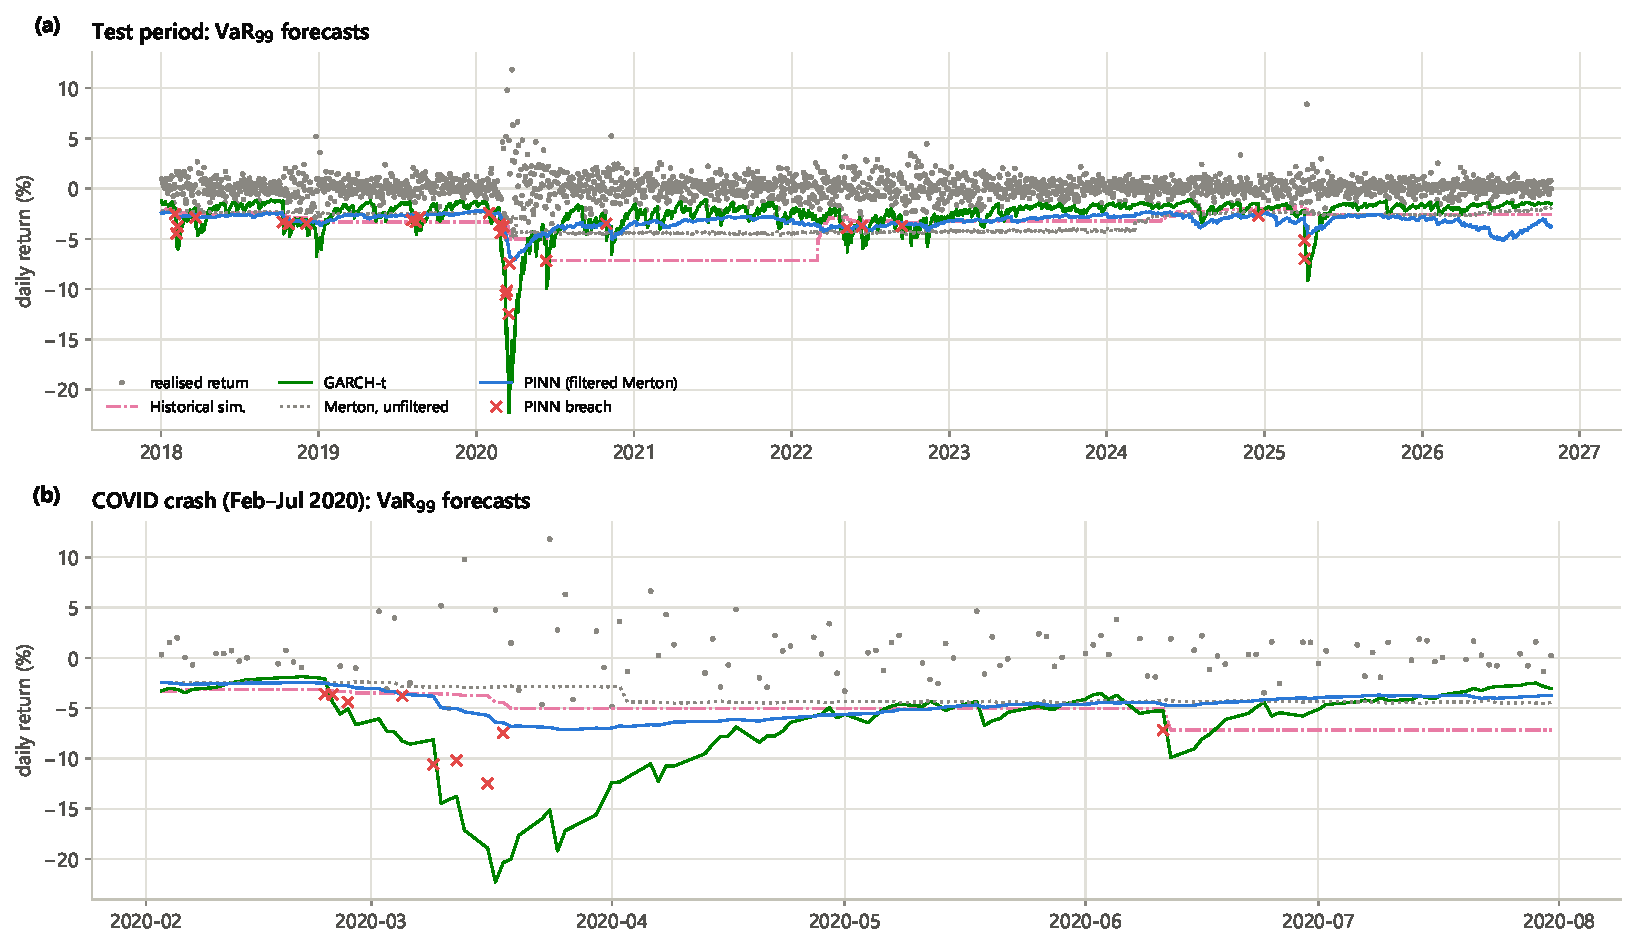
\includegraphics[width=\linewidth]{stage6_realdata_sp/fig03_var_paths.pdf}
  \caption{S\&P basket: daily 99\% VaR forecasts of the PINN and benchmarks against realised returns,
    2018--2026.}
  \label{fig:varpaths}
\end{figure}

% ------------------------------------------------------------------------------------------------
\section{Physics versus data, and failure cases (RQ3)}
\label{sec:res-ablation}

\subsection{Physics-informed versus data-only}
To isolate the contribution of the physics, the PINN was compared with a \emph{data-only} network that is
identical in architecture, optimiser, learning-rate schedule, number of steps and normaliser estimator, but
is trained by maximum likelihood on $N$ exact samples instead of the PIDE. The samples are spread over 16
times in $[t_0, T]$, 20\% are held out for early stopping, and $N$ ranges from $10^3$ to $10^6$ with three
seeds each. Monte Carlo on the same samples is the third method, and all models are weighted on the same
importance draws, so differences between them are model differences.

\begin{table}[t]
  \centering
  \caption{Physics versus data: median ES$_{99}$ error over 20 portfolios (data-only and Monte Carlo:
    median over three seeds). The PINN uses no samples
    (\texttt{results/stage7\_physics\_vs\_data\_d*/metrics.json}).}
  \label{tab:physdata}
  \begin{tabular}{llccc@{\hspace{2em}}ccc}
    \toprule
    & & \multicolumn{3}{c}{$d = 2$} & \multicolumn{3}{c}{$d = 5$} \\
    Method & $N$ & 1 day & 5 days & 10 days & 1 day & 5 days & 10 days \\
    \midrule
    PINN (physics)   & 0       & 1.3\% & 0.9\% & 0.08\% & 1.8\% & 2.2\% & 0.8\% \\
    \midrule
    \multirow{4}{*}{Data-only NN}
      & $10^3$ & 21\%  & 4.7\% & 1.7\% & 44\% & 28\% & 64\% \\
      & $10^4$ & 13\%  & 2.1\% & 3.8\% & 13\% & 5.7\% & 9.2\% \\
      & $10^5$ & 5.0\% & 0.8\% & 2.5\% & 3.3\% & 1.8\% & 3.2\% \\
      & $10^6$ & 1.3\% & 0.4\% & 0.18\% & 2.8\% & 0.8\% & 0.8\% \\
    \midrule
    \multirow{4}{*}{MC, same samples}
      & $10^3$ & 75\% & 16\% & 34\% & 68\% & 32\% & 23\% \\
      & $10^4$ & 23\% & 7.1\% & 9.7\% & 11\% & 8.1\% & 6.0\% \\
      & $10^5$ & 7.8\% & 5.2\% & 1.6\% & 11\% & 3.2\% & 1.5\% \\
      & $10^6$ & 0.8\% & 1.2\% & 1.1\% & 2.1\% & 0.7\% & 1.6\% \\
    \bottomrule
  \end{tabular}
\end{table}

\Cref{tab:physdata} and \cref{fig:physdata} give the answer to RQ3. The PINN, which sees no samples, is worth
roughly $10^5$ to $10^6$ exact samples. The data-only network reaches the PINN's 5-day error at about
$6.6\times10^4$ samples in both dimensions; at 1 and 10 days it does not reach it before $10^6$. With the sample
sizes available in practice (a few thousand daily observations), data-only errors are 5--60\%. The data-only
network is itself better than Monte Carlo on the same samples at small $N$, since it smooths across times, but
both need of order $10^6$ samples to reach the accuracy the physics provides for free.

This comparison should be read with one caveat. When the model is known, one can always simulate, so the
PINN's advantage is not that samples are unavailable. Its advantage is that one training run gives a smooth,
normalised and differentiable density at every time in $[t_0, T]$, which can be amortised over parameters
(\cref{sec:res-amortised}) and differentiated for risk contributions, at no sampling cost per query.

\begin{figure}[t]
  \centering
  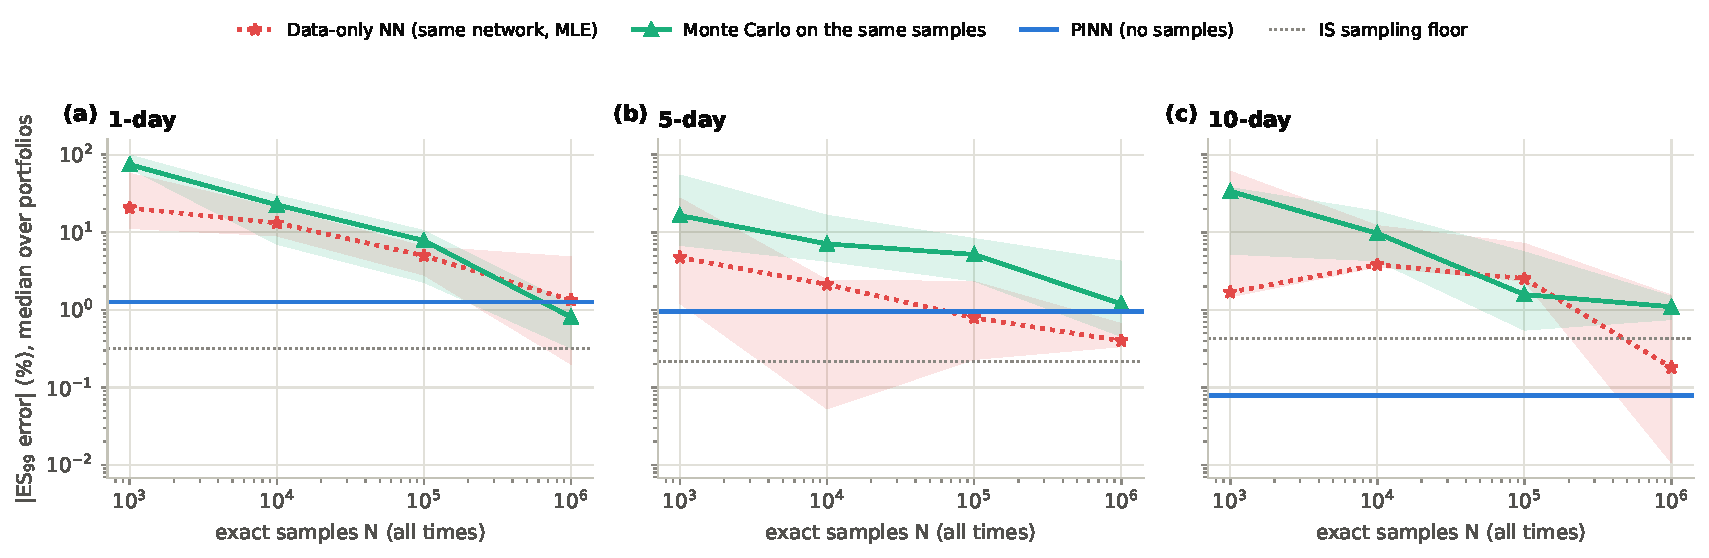
\includegraphics[width=\linewidth]{stage7_physics_vs_data_d2/fig02_es_vs_samples.pdf}
  \caption{$d = 2$: ES$_{99}$ error against the number of exact samples for the data-only network (red) and
    Monte Carlo on the same samples (green); the PINN uses none (blue line). Bands: range over seeds.}
  \label{fig:physdata}
\end{figure}

\subsection{Failure cases}
\label{sec:res-failure}
Three controlled changes to the $d = 2$ setup test the method's assumptions, and two failures from earlier
stages are collected with them (\cref{tab:failure}, \cref{fig:failure}).

\begin{table}[t]
  \centering
  \caption{Failure cases: median ES$_{99}$ error over portfolios
    (\texttt{results/stage7\_final/failure\_cases.csv}).}
  \label{tab:failure}
  \begin{tabular}{lccc}
    \toprule
    Case & 1 day & 5 days & 10 days \\
    \midrule
    $d = 2$, Stage 4 reference                    & 0.70\% & 0.69\% & 0.99\% \\
    $\lambda = 50$/yr, proposal $k \le 3$ jumps    & 0.59\% & 0.74\% & 0.78\% \\
    $\lambda = 50$/yr, proposal $k \le 10$ jumps   & 0.29\% & 0.07\% & 0.12\% \\
    $t_0 = 0.05$ day                               & \textbf{5.2\%} & 0.94\% & 0.25\% \\
    $d = 5$ amortised, worst $\theta$ (Stage 5)    & 3.6\% & 4.7\% & \textbf{10\%} \\
    $d = 10$ (Stage 4)                             & \textbf{5.2\%} & \textbf{44\%} & \textbf{62\%} \\
    \bottomrule
  \end{tabular}
\end{table}

\paragraph{High jump intensity.} At $\lambda = 50$/yr the default proposal covers at most three jumps, while
the probability of more jumps reaches 14\% at 10 days. Contrary to the expectation, the PINN does not break:
the error stays below 1\%, because the residual loss still trains the network where the proposal is thin.
Widening the proposal to ten jumps reduces the error by a factor of five to ten. The jump coverage of the
proposal is therefore a tuning choice, not a hard limit.

\paragraph{Short start time.} Starting at $t_0 = 0.05$ day instead of 0.5 day makes the initial density ten
times sharper. This is a genuine failure at short horizons: the 1-day ES$_{99}$ error is 5.2\%, the 1-day VaR$_{99}$
error 21\%, and the tail log-density error 0.13 (0.02 for the reference). The error decays as the density
widens, to 0.25\% at 10 days. Short horizons need either a $t_0$ close to the first horizon of interest or a
time rescaling that keeps the initial density resolvable.

\paragraph{Dimension and parameter range.} The $d = 10$ breakdown (\cref{sec:res-scaling}) and the worst corner
of the $d = 5$ amortised box (\cref{sec:res-amortised}) are the largest errors in the study. Both grow with
horizon, so they come from error accumulating along the time direction rather than from the initial condition.

\paragraph{Far-tail extrapolation.} \Cref{fig:failure}(b) traces $\log p - \log q$ along rays from the centre.
For the exact density it falls to between $-50$ and $-230$ at 150 whitened units; for the PINN it turns positive
beyond about 20 units and keeps rising. Outside the trained region the network decays more slowly than the
heavy-tailed proposal, so a single far-out draw can carry all the importance weight. This is the mechanism behind
the S\&P blow-up in \cref{sec:res-real}, and it justifies the trust region used there. The PINN's density is
reliable only within the region covered by its collocation points.

\begin{figure}[t]
  \centering
  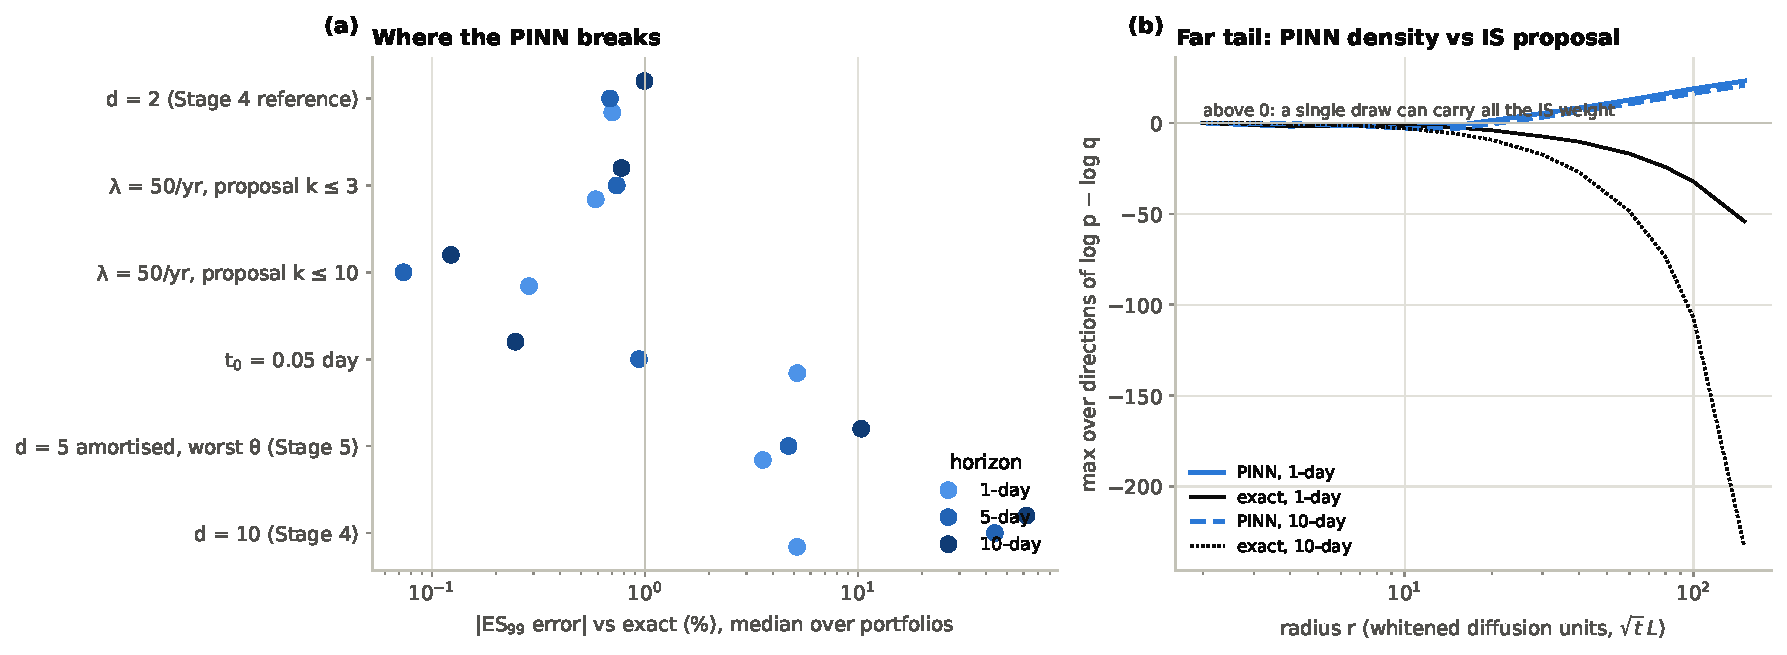
\includegraphics[width=\linewidth]{stage7_final/fig02_failure_cases.pdf}
  \caption{(a) ES$_{99}$ error by failure case and horizon; the vertical line marks 1\%. (b) Far-tail probe:
    the maximum over 2,000 directions of $\log p - \log q$ for the PINN and the exact density.}
  \label{fig:failure}
\end{figure}

% ------------------------------------------------------------------------------------------------
\section{Summary and answers to the research questions}
\label{sec:res-summary}

\Cref{fig:scorecard} places the PINN's ES$_{99}$ error next to its baseline in every stage.

\begin{figure}[t]
  \centering
  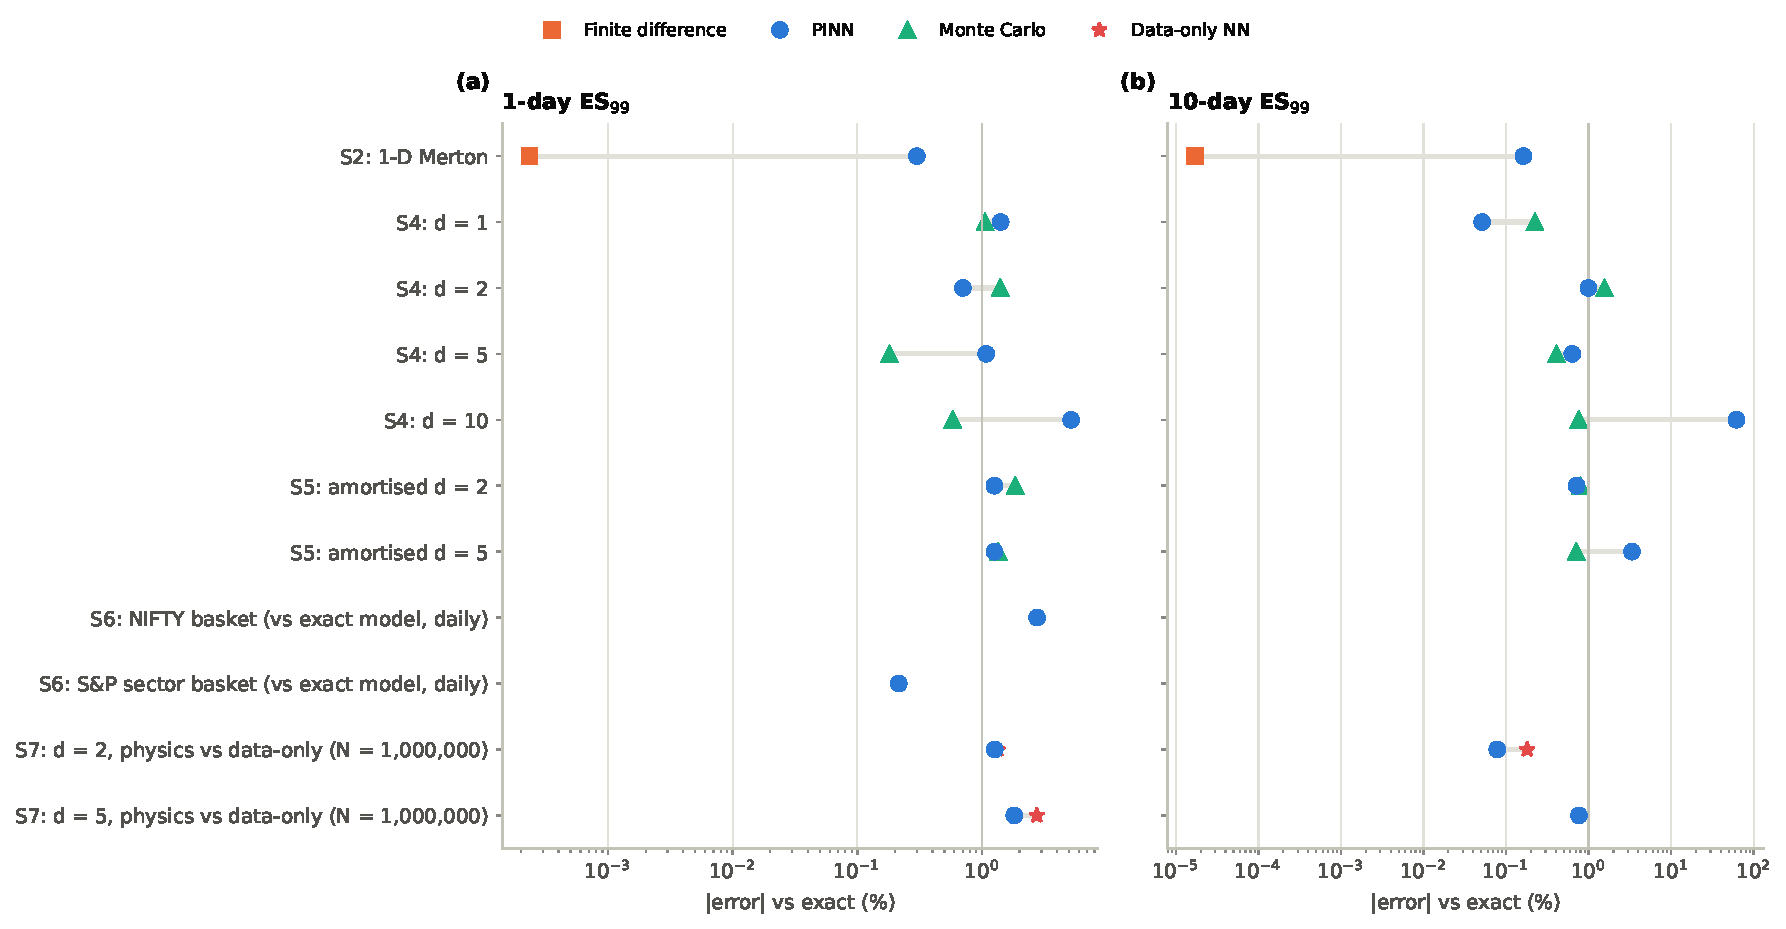
\includegraphics[width=\linewidth]{stage7_final/fig01_scorecard.pdf}
  \caption{Scorecard over Stages 2--7: PINN ES$_{99}$ error (blue) against the baseline of each stage
    (FD, Monte Carlo at the same budget, or the data-only network), at 1 and 10 days.}
  \label{fig:scorecard}
\end{figure}

\begin{description}
  \item[RQ1 (bulk versus tail).] With the log-form residual the tail is learned as accurately as the bulk:
    tail log-density errors are 0.015--0.05 for $d \le 5$, and ES errors are at or below 1\%. The tail fails
    first at the limits: at $d = 10$ (tail error 0.20), for a very sharp initial density, and beyond the
    collocation region, where the density is not constrained at all.
  \item[RQ2 (calibration on real data).] The PINN reproduces the filtered Merton model to within 0.2--2.8\%
    in daily ES with identical breaches. The model passes unconditional coverage at 99\% on both markets but is
    conservative at 97.5\%, and on the FZ0 score it is beaten by FHS, DCC, GARCH-$t$ and EVT while beating
    Gaussian, HS and unfiltered Merton.
  \item[RQ3 (physics versus data).] The physics replaces roughly $10^5$--$10^6$ exact samples. At realistic
    sample sizes a data-only network of the same design is 5--60\% off.
  \item[RQ4 (scaling).] One architecture and training budget works up to $d = 5$ at about 1\% error, with
    training time nearly flat in $d$, where grid methods are already impractical beyond $d = 3$. It breaks at
    $d = 10$.
  \item[RQ5 (latency).] A single amortised network answers queries over the whole parameter box in 4--18\,ms,
    with sensitivities by differentiation. For the Merton model Monte Carlo is faster at matched error, so there
    is no break-even; a speed advantage requires models whose simulation is expensive.
\end{description}

\paragraph{Limitations.} All synthetic results use a model with a common jump factor, which keeps the jump
integral one-dimensional; idiosyncratic jumps would need a $d$-dimensional integral. The multi-asset method was
not made to work at $d = 10$. The real-data comparison tests the jump-diffusion model as much as the PINN, and
the volatility filter, not the PINN, determines most of the backtest result.

\chapter{Conclusion}
\label{ch:conclusion}

\section{Summary}
This thesis tested whether physics-informed neural networks give accurate and useful tail-risk estimates under
jump-diffusion dynamics, against an exact reference at every step. The answer depends on the setting, and the
study can say where the PINN helps and where it does not.

In one dimension a carefully designed PINN learns the density and its tail to within 1\% in VaR and ES at every
level tested. The design matters more than the network: writing the residual for the log density, resolving the
jump integral with enough quadrature nodes and penalising the normalisation each change the tail error by an order
of magnitude, while tail-adaptive sampling does not help. In one dimension, however, finite differences are faster
and far more accurate, so the 1-D study validates the method rather than motivating it.

The method carries over to several assets without a grid. Collocation, normalisation and risk all use one proposal
built from the equation's coefficients, and the Laplacian can be estimated stochastically. With one architecture and
training budget the ES error stays near 1\% up to five assets, with training time almost independent of the
dimension, in a regime where finite differences are already impractical. At ten assets the method breaks.

An amortised network that takes the volatility level, jump intensity and jump mean as inputs covers a whole range of
market states with one training run and provides risk contributions and scenario curves by differentiation. For the
Merton model, though, Monte Carlo is faster at matched error, because exact simulation is cheap; the PINN does not pay
back its training cost in latency.

On real data the PINN reproduces its jump-diffusion model closely, with daily ES within 0.2--2.8\% of the exact model
and identical breaches. Its backtest performance is therefore that of the model: better than Gaussian, historical
simulation and unfiltered jump-diffusion forecasts, conservative at 97.5\%, and behind the best volatility-filtered
models (filtered historical simulation, DCC, GARCH-$t$, EVT).

The physics is worth a great deal of data. Trained on no samples, the PINN matches a network of identical design
trained on $10^5$ to $10^6$ exact samples; with the few thousand observations available in practice, the data-only
network is 5--60\% off.

\section{Answers to the research questions}
\begin{description}
  \item[RQ1.] With the log-form residual the tail is learned as accurately as the bulk for up to five assets. The tail
    is where the method fails first: in ten dimensions, for a very sharp initial density, and outside the region
    covered by training points.
  \item[RQ2.] Against exact values, ES errors are about 1\% up to five assets. On real data the PINN is a faithful
    surrogate of its model, and calibration is determined by the model, not by the network.
  \item[RQ3.] The equation replaces $10^5$--$10^6$ exact samples.
  \item[RQ4.] The method scales to five assets at roughly constant cost and accuracy and breaks at ten with the
    architecture and budget used here.
  \item[RQ5.] One network answers queries over a parameter box in milliseconds, but for the Merton model Monte Carlo
    is faster at equal error, and there is no break-even.
\end{description}

\section{Practical implications}
\begin{itemize}
  \item A PINN is worth using when the model is expensive to simulate, when a smooth and differentiable density is
    needed (risk contributions, scenario analysis, calibration), or when one model must serve many parameter
    values. For a model as simple as Merton with linear portfolios, Monte Carlo or the closed form is the better tool.
  \item A neural density must not be trusted outside the region where it was trained. Importance-sampling estimates
    should use a trust region, as in the real-data study, or a proposal whose tails are lighter than the network's.
  \item Model risk dominates network error in practice: on real data the choice of model and volatility filter
    mattered more for the backtests than the difference between the PINN and the exact density.
\end{itemize}

\section{Limitations}
\begin{itemize}
  \item All synthetic results use one common jump factor, which keeps the jump integral one-dimensional.
    Idiosyncratic jumps would make it $d$-dimensional and are untested.
  \item Volatility enters only as a daily scale; stochastic volatility, which would double the state dimension, is
    not modelled.
  \item The method was not made to work at ten assets, and the amortised model degrades at long horizons in five.
  \item The initial condition is the exact short-time density; in models without a closed form it would have to be
    approximated, adding an error that this study does not measure.
  \item The real-data evaluation covers two five-asset baskets and one test period (2018--2026).
\end{itemize}

\section{Future work}
\begin{itemize}
  \item \textbf{Higher dimensions:} wider networks and longer training, time-marching (training successive time
    windows), and separable or low-rank architectures, to move the breakdown point beyond ten assets.
  \item \textbf{Richer models:} stochastic volatility (Bates), idiosyncratic jumps and self-exciting (Hawkes) jump
    arrivals. These are also the models where simulation is expensive and the PINN could win on latency.
  \item \textbf{Option-implied calibration:} fitting the jump parameters to option prices, so that the tail reflects
    the market's forward-looking view.
  \item \textbf{Uncertainty quantification:} ensembles or Bayesian PINNs to attach an error bar to each risk estimate,
    which would also detect the far-tail extrapolation failure automatically.
  \item \textbf{Short horizons:} a time rescaling that keeps the initial density resolvable, to remove the
    short-start-time failure.
\end{itemize}


\bibliographystyle{IEEEtranN}
\bibliography{references}

\end{document}
